\documentclass[oneside,a4paper,12pt, headings=normal, oneside, hidelinks, scrreprt]{normas-utf-tex}
\usepackage[alf,abnt-emphasize=bf,bibjustif,recuo=0cm,abnt-etal-cite=2]{abntcite}
\usepackage{indentfirst}
\usepackage{latexsym,amsmath,amssymb,amsfonts,amsthm}
\usepackage{url}
\usepackage{graphicx}
\usepackage[brazil]{babel}
\usepackage{gensymb}
\usepackage[table]{xcolor}
\definecolor{verde}{rgb}{0.25,0.5,0.35}
\definecolor{jpurple}{rgb}{0.5,0,0.35}
\usepackage{listings}
\usepackage[utf8]{inputenc}
\usepackage{listingsutf8}


\usepackage{color}
    \definecolor{editorGray}{rgb}{0.95, 0.95, 0.95}
    \definecolor{editorOcher}{rgb}{1, 0.5, 0} % #FF7F00 -> rgb(239, 169, 0)
    \definecolor{editorGreen}{rgb}{0, 0.5, 0} % #007C00 -> rgb(0, 124, 0)
    \usepackage{upquote}
    \usepackage{listings}
    \lstdefinelanguage{JavaScript}{
      morekeywords={break, case, catch, continue, debugger, default, delete,         do, else, false, finally, for, function, if, in, instanceof, new, null, return, switch, this, throw, true, try, typeof, var, void, while, with},
      morecomment=[s]{/*}{*/},
      morecomment=[l]//,
      morestring=[b]",
      morestring=[b]'
    }
    \lstdefinelanguage{CSS}{
      keywords={accelerator,azimuth,background,background-attachment,
            background-color,background-image,background-position,
            background-position-x,background-position-y,background-repeat,
            behavior,border,border-bottom,border-bottom-color,
            border-bottom-style,border-bottom-width,border-collapse,
            border-color,border-left,border-left-color,border-left-style,
            border-left-width,border-right,border-right-color,
            border-right-style,border-right-width,border-spacing,
            border-style,border-top,border-top-color,border-top-style,
            border-top-width,border-width,bottom,caption-side,clear,
            clip,color,content,counter-increment,counter-reset,cue,
            cue-after,cue-before,cursor,direction,display,elevation,
            empty-cells,filter,float,font,font-family,font-size,
            font-size-adjust,font-stretch,font-style,font-variant,
            font-weight,height,ime-mode,include-source,
            layer-background-color,layer-background-image,layout-flow,
            layout-grid,layout-grid-char,layout-grid-char-spacing,
            layout-grid-line,layout-grid-mode,layout-grid-type,left,
            letter-spacing,line-break,line-height,list-style,
            list-style-image,list-style-position,list-style-type,margin,
            margin-bottom,margin-left,margin-right,margin-top,
            marker-offset,marks,max-height,max-width,min-height,
            min-width,-moz-binding,-moz-border-radius,
            -moz-border-radius-topleft,-moz-border-radius-topright,
            -moz-border-radius-bottomright,-moz-border-radius-bottomleft,
            -moz-border-top-colors,-moz-border-right-colors,
            -moz-border-bottom-colors,-moz-border-left-colors,-moz-opacity,
            -moz-outline,-moz-outline-color,-moz-outline-style,
            -moz-outline-width,-moz-user-focus,-moz-user-input,
            -moz-user-modify,-moz-user-select,orphans,outline,
            outline-color,outline-style,outline-width,overflow,
            overflow-X,overflow-Y,padding,padding-bottom,padding-left,
            padding-right,padding-top,page,page-break-after,
            page-break-before,page-break-inside,pause,pause-after,
            pause-before,pitch,pitch-range,play-during,position,quotes,
            -replace,richness,right,ruby-align,ruby-overhang,
            ruby-position,-set-link-source,size,speak,speak-header,
            speak-numeral,speak-punctuation,speech-rate,stress,
            scrollbar-arrow-color,scrollbar-base-color,
            scrollbar-dark-shadow-color,scrollbar-face-color,
            scrollbar-highlight-color,scrollbar-shadow-color,
            scrollbar-3d-light-color,scrollbar-track-color,table-layout,
            text-align,text-align-last,text-decoration,text-indent,
            text-justify,text-overflow,text-shadow,text-transform,
            text-autospace,text-kashida-space,text-underline-position,top,
            unicode-bidi,-use-link-source,vertical-align,visibility,
            voice-family,volume,white-space,widows,width,word-break,
            word-spacing,word-wrap,writing-mode,z-index,zoom},  
      sensitive=true,
      morecomment=[l]{//},
      morecomment=[s]{/*}{*/},
      morestring=[b]',
      morestring=[b]",
      alsoletter={:},
      alsodigit={-}
    }
    \lstdefinelanguage{HTML5}{
            language=html,
            sensitive=true, 
            alsoletter={<>=-},
            otherkeywords={
            % HTML tags
            <, </, >,
            </a, <a, </a>,
            </abbr, <abbr, </abbr>,
            </address, <address, </address>,
            </area, <area, </area>,
            </area, <area, </area>,
            </article, <article, </article>,
            </aside, <aside, </aside>,
            </audio, <audio, </audio>,
            </audio, <audio, </audio>,
            </b, <b, </b>,
            </base, <base, </base>,
            </bdi, <bdi, </bdi>,
            </bdo, <bdo, </bdo>,
            </blockquote, <blockquote, </blockquote>,
            </body, <body, </body>,
            </br, <br, </br>,
            </button, <button, </button>,
            </canvas, <canvas, </canvas>,
            </caption, <caption, </caption>,
            </cite, <cite, </cite>,
            </code, <code, </code>,
            </col, <col, </col>,
            </colgroup, <colgroup, </colgroup>,
            </data, <data, </data>,
            </datalist, <datalist, </datalist>,
            </dd, <dd, </dd>,
            </del, <del, </del>,
            </details, <details, </details>,
            </dfn, <dfn, </dfn>,
            </div, <div, </div>,
            </dl, <dl, </dl>,
            </dt, <dt, </dt>,
            </em, <em, </em>,
            </embed, <embed, </embed>,
            </fieldset, <fieldset, </fieldset>,
            </figcaption, <figcaption, </figcaption>,
            </figure, <figure, </figure>,
            </footer, <footer, </footer>,
            </form, <form, </form>,
            </h1, <h1, </h1>,
            </h2, <h2, </h2>,
            </h3, <h3, </h3>,
            </h4, <h4, </h4>,
            </h5, <h5, </h5>,
            </h6, <h6, </h6>,
            </head, <head, </head>,
            </header, <header, </header>,
            </hr, <hr, </hr>,
            </html, <html, </html>,
            </i, <i, </i>,
            </iframe, <iframe, </iframe>,
            </img, <img, </img>,
            </input, <input, </input>,
            </ins, <ins, </ins>,
            </kbd, <kbd, </kbd>,
            </keygen, <keygen, </keygen>,
            </label, <label, </label>,
            </legend, <legend, </legend>,
            </li, <li, </li>,
            </link, <link, </link>,
            </main, <main, </main>,
            </map, <map, </map>,
            </mark, <mark, </mark>,
            </math, <math, </math>,
            </menu, <menu, </menu>,
            </menuitem, <menuitem, </menuitem>,
            </meta, <meta, </meta>,
            </meter, <meter, </meter>,
            </nav, <nav, </nav>,
            </noscript, <noscript, </noscript>,
            </object, <object, </object>,
            </ol, <ol, </ol>,
            </optgroup, <optgroup, </optgroup>,
            </option, <option, </option>,
            </output, <output, </output>,
            </p, <p, </p>,
            </param, <param, </param>,
            </pre, <pre, </pre>,
            </progress, <progress, </progress>,
            </q, <q, </q>,
            </rp, <rp, </rp>,
            </rt, <rt, </rt>,
            </ruby, <ruby, </ruby>,
            </s, <s, </s>,
            </samp, <samp, </samp>,
            </script, <script, </script>,
            </section, <section, </section>,
            </select, <select, </select>,
            </small, <small, </small>,
            </source, <source, </source>,
            </span, <span, </span>,
            </strong, <strong, </strong>,
            </style, <style, </style>,
            </summary, <summary, </summary>,
            </sup, <sup, </sup>,
            </svg, <svg, </svg>,
            </table, <table, </table>,
            </tbody, <tbody, </tbody>,
            </td, <td, </td>,
            </template, <template, </template>,
            </textarea, <textarea, </textarea>,
            </tfoot, <tfoot, </tfoot>,
            </th, <th, </th>,
            </thead, <thead, </thead>,
            </time, <time, </time>,
            </title, <title, </title>,
            </tr, <tr, </tr>,
            </track, <track, </track>,
            </u, <u, </u>,
            </ul, <ul, </ul>,
            </var, <var, </var>,
            </video, <video, </video>,
            </wbr, <wbr, </wbr>,
            />, <!
            },  
            ndkeywords={
            % General
            =,
            % HTML attributes
            accept=, accept-charset=, accesskey=, action=, align=, alt=, async=, autocomplete=, autofocus=, autoplay=, autosave=, bgcolor=, border=, buffered=, challenge=, charset=, checked=, cite=, class=, code=, codebase=, color=, cols=, colspan=, content=, contenteditable=, contextmenu=, controls=, coords=, data=, datetime=, default=, defer=, dir=, dirname=, disabled=, download=, draggable=, dropzone=, enctype=, for=, form=, formaction=, headers=, height=, hidden=, high=, href=, hreflang=, http-equiv=, icon=, id=, ismap=, itemprop=, keytype=, kind=, label=, lang=, language=, list=, loop=, low=, manifest=, max=, maxlength=, media=, method=, min=, multiple=, name=, novalidate=, open=, optimum=, pattern=, ping=, placeholder=, poster=, preload=, pubdate=, radiogroup=, readonly=, rel=, required=, reversed=, rows=, rowspan=, sandbox=, scope=, scoped=, seamless=, selected=, shape=, size=, sizes=, span=, spellcheck=, src=, srcdoc=, srclang=, start=, step=, style=, summary=, tabindex=, target=, title=, type=, usemap=, value=, width=, wrap=,
            % CSS properties
            accelerator:,azimuth:,background:,background-attachment:,
            background-color:,background-image:,background-position:,
            background-position-x:,background-position-y:,background-repeat:,
            behavior:,border:,border-bottom:,border-bottom-color:,
            border-bottom-style:,border-bottom-width:,border-collapse:,
            border-color:,border-left:,border-left-color:,border-left-style:,
            border-left-width:,border-right:,border-right-color:,
            border-right-style:,border-right-width:,border-spacing:,
            border-style:,border-top:,border-top-color:,border-top-style:,
            border-top-width:,border-width:,bottom:,caption-side:,clear:,
            clip:,color:,content:,counter-increment:,counter-reset:,cue:,
            cue-after:,cue-before:,cursor:,direction:,display:,elevation:,
            empty-cells:,filter:,float:,font:,font-family:,font-size:,
            font-size-adjust:,font-stretch:,font-style:,font-variant:,
            font-weight:,height:,ime-mode:,include-source:,
            layer-background-color:,layer-background-image:,layout-flow:,
            layout-grid:,layout-grid-char:,layout-grid-char-spacing:,
            layout-grid-line:,layout-grid-mode:,layout-grid-type:,left:,
            letter-spacing:,line-break:,line-height:,list-style:,
            list-style-image:,list-style-position:,list-style-type:,margin:,
            margin-bottom:,margin-left:,margin-right:,margin-top:,
            marker-offset:,marks:,max-height:,max-width:,min-height:,
            min-width:,transition-duration:,transition-property:,
            transition-timing-function:,transform:,
            -moz-transform:,-moz-binding:,-moz-border-radius:,
            -moz-border-radius-topleft:,-moz-border-radius-topright:,
            -moz-border-radius-bottomright:,-moz-border-radius-bottomleft:,
            -moz-border-top-colors:,-moz-border-right-colors:,
            -moz-border-bottom-colors:,-moz-border-left-colors:,-moz-opacity:,
            -moz-outline:,-moz-outline-color:,-moz-outline-style:,
            -moz-outline-width:,-moz-user-focus:,-moz-user-input:,
            -moz-user-modify:,-moz-user-select:,orphans:,outline:,
            outline-color:,outline-style:,outline-width:,overflow:,
            overflow-X:,overflow-Y:,padding:,padding-bottom:,padding-left:,
            padding-right:,padding-top:,page:,page-break-after:,
            page-break-before:,page-break-inside:,pause:,pause-after:,
            pause-before:,pitch:,pitch-range:,play-during:,position:,quotes:,
            -replace:,richness:,right:,ruby-align:,ruby-overhang:,
            ruby-position:,-set-link-source:,size:,speak:,speak-header:,
            speak-numeral:,speak-punctuation:,speech-rate:,stress:,
            scrollbar-arrow-color:,scrollbar-base-color:,
            scrollbar-dark-shadow-color:,scrollbar-face-color:,
            scrollbar-highlight-color:,scrollbar-shadow-color:,
            scrollbar-3d-light-color:,scrollbar-track-color:,table-layout:,
            text-align:,text-align-last:,text-decoration:,text-indent:,
            text-justify:,text-overflow:,text-shadow:,text-transform:,
            text-autospace:,text-kashida-space:,text-underline-position:,top:,
            unicode-bidi:,-use-link-source:,vertical-align:,visibility:,
            voice-family:,volume:,white-space:,widows:,width:,word-break:,
            word-spacing:,word-wrap:,writing-mode:,z-index:,zoom:
            },  
            morecomment=[s]{<!--}{-->},
            tag=[s]
    }

    \lstset{%
        % Basic design
        backgroundcolor=\color{editorGray},
        basicstyle={\ttfamily\footnotesize},   %reduzir o tamanho da fonte
        frame=l,
        % Line numbers
        xleftmargin={0.2cm},
        numbers=left,
        stepnumber=1,
        firstnumber=1,
        numberfirstline=true,
        % Code design   
        keywordstyle=\color{blue}\bfseries,
        commentstyle=\color{darkgray}\ttfamily,
        ndkeywordstyle=\color{editorGreen}\bfseries,
        stringstyle=\color{editorOcher},
        % Code
        language=HTML5,
        alsodigit={.:;},
        tabsize=2,
        showtabs=false,
        showspaces=false,
        showstringspaces=false,
        extendedchars=true,
        breaklines=true,        
    }
%=======================================================================
%Informações Gerais (a serem preenchidas pelo aluno)
%=======================================================================

%======Instituição e programa
\instituicao{Universidade Tecnológica Federal do Paraná}
%\departamento{Câmpus Guarapuava}
\programa{Tecnologia em Sistemas para Internet}

%======Orientador e Co-orientador (caso necessario)
%\orientador {Prof. Dr. Eleandro Maschio e Prof. Dr. Diego Marczal}

%======Alterar o tipo do documento de acordo com a necessidade. 
\documento{Projeto Desenvolvimento para Web II}

%======Nome para citacoes. Ex: PORFIRIO, Andres.
\cita{CAMPOS, Ester de Arruda; CAVALCANTI, Marcus Vinicius}
%======Autor principal
\autor{CAMPOS, Ester de Arruda}
\autordois{Cavalcanti, Marcus Vinicius}
%use se necessário

%======Título do trabalho (Português e Inglês)
\titulo{Tema: Fotos}
\title{Work Title}

%======Palavras Chave (Português e Inglês)
\palavraschave{Web II, Javascript, JQuery, HTML, CSS}
\keywords{Web II, Javascript, JQuery, HTML, CSS}

%======Comentário da folha de rosto.
%Este texto pode ser personalizado de acordo com as exigências.
\comentario{Projeto apresentado ao professor Dr. Roni Fabio Banaszewski como requisito parcial para composição de nota semestral de sua respectivas disciplina – Desenvolvimento para Web II.
}

%======Local e data
\local{Guarapuava}
\data{\the\year}


%=======================================================================
%Início do documento
%=======================================================================

\begin{document}

\lstset{inputencoding=utf8/latin1}
\clearpage
\pagenumbering{arabic}

%--------------------------------------
%Elementos Pré-Textuais
%--------------------------------------

\capa

\folhaderosto

%ficha catalográfica: deve ser impressa separadamente no verso da folha de rosto. somente para a versão final do documento (biblioteca).


%\begin{resumo}
%	%Exemplo de resumo

Resumo.

O Problema das Oito Rainhas consiste no desafio lógico de dispor oito peças (rainha) em um tabuleiro de xadrez (tradicional, $8x8$) de forma que nenhuma peça seja atacada por outra. Assim, faz-se necessário que duas rainhas quaisquer não estejam numa mesma linha, coluna ou diagonal. O problema possui 92 soluções distintas que na realidade tratam-se de 12 soluções originais de onde obtemos as outras soluções por operações de simetria (rotação e reflexão). O presente projeto apresentará um aplicativo que gerencia a colocação das oito damas/rainhas, uma por vez, no tabuleiro de xadrez. O jogador poderá inserir e retirar cada rainha deste tabuleiro mediante coordenadas (que vão de “$a$” até “$h$” e de $1$ até $8$, conforme o padrão internacional). A cada movimento, constatará e informará ao jogador onde ocorreu o primeiro ataque. Sinalizaremos quando o problema for resolvido. Frisamos que este aplicativo não irá catalogar as 92 possíveis soluções, mas verificar se o estágio atual de resolução condiz com as restrições do problema proposto.
%\end{resumo}

%\begin{abstract}
%	The Problem of Eight Queens is the logical challenge to have eight pieces (queens) on a chessboard (traditional $8x8 $) so that no is attacked by another. Thus, it is necessary that any two queens are not in the same row, column or diagonal. The problem has 92 distinct solutions that in fact these are 12 unique solutions where we get the other solutions by symmetry operations (rotation and reflection). This project will submit an application that manages the placement of the eight queens, one at a time on the chessboard. The player can insert and remove each queen of this board by coordinates (ranging from "$a$"  to  "$h$" and $1$ to $8$, as the international standard). Every movement, see and tell the player where the first attack occurred. Sinalizaremos when the problem is resolved. We stress that this application will not catalog the 92 possible solutions, but check if the current stage of resolution consistent with the restrictions of the proposed problem.

%\end{abstract}


%Listas. Obrigatório quando constar no desenvolvimento do trabalho. Consultar o documento das normas da ABNT para maiores detalhes.
\listadefiguras
%\listadetabelas
%\listadesiglas
%\listadesimbolos

\sumario

%--------------------------------------
%Texto
%--------------------------------------

%Incluir arquivos .tex da pasta src/

\chapter{Introdução}

\section{Justificativa}
	
	

\section{Objetivo}

	O presente projeto tem por objetivo apresentar 

\section{Estrutura do projeto} 

	O Capítulo 1 – Introdução, irá definir o que vem a ser o projeto e quais os objetivos a serem analisados. No Capítulo 2, estaremos apresentando as exigências Gerais definidas como requisito para elaboração do projeto. O Capítulo 3, apresentará respostas para as exigências específicas e seus devidos tópicos. Por fim, no Capítulo 4 apresentaremos alguns trechos de código.
		
	Toda formatação para este texto incluindo a formatação para apresentação dos códigos elaborados foram feitos utilizando a linguagem $LaTeX$.


\section{ Metodologia utilizada}
	Utilizaremos o método de pesquisa aplicada cuja meta é contribuir para fins práticos buscando solução para problema concreto.



\chapter{Exigências Gerais}
\section{Conteúdo}

	O conteúdo do site é de autoria pessoal. Todas as fotos são do portfólio da fotografa a mesma disponibiliza e cede os direitos de utilização de imagens para este projeto, com citação.

\section{HTML5 e CSS}

	Neste projeto foram utilizados $HTML5$ e $CSS$ um dos exemplos para utilização da $CSS$ podem ser conferidos no item $Layout$
	
     
\section{Framework}

	Foi utilizado o framework Bootstrap seguindo uma das recomendações.

\section{Layout}
	Conforme indicado pelo docente uma das páginas do projeto precisa ser totalmente responsiva. Desta forma apresentamos a página $index.html$.
	
	Não utilizamos $templates$ prontos. Nesta página fazemos utilização de $CSS$.
	
\begin{lstlisting}
<link href="assets/libs/bootstrap/css/bootstrap.css" rel="stylesheet">
<link href="assets/resources/css/principal.css" rel="stylesheet">
<link href="assets/resources/css/home.css" rel="stylesheet">
\end{lstlisting}	
	
	Esta tela é o primeiro contato que um cliente que esteja visitando a página terá. Por este motivo pensamos em mostrar algumas imagens para que o visitante tenha a sensação de que está no lugar certo. 
	
	Desta forma deixamos na página inicial apenas um $slider$ onde são apresentadas cinco (5) fotos. Este $slider$ foi montado para apresentar uma transição de fotos de maneira simples. O intervalo entre uma foto e outra é feito de modo que apareça um efeito de opacidade.
	
	O efeito de opacidade e transição foi conseguido utilizando $CSS$ $transitions$ seguindo algumas ideias de Rich Bradshaw em seu site \cite{RichBradshaw}.

\subsubsection{HTML e CSS}	
	
	Criamos um arquivo chamado $home.css$ onde estão as configurações $crossfade$ do $css$. São estas configurações as responsáveis pelos efeitos de transição/animação das $5$ imagens. Este efeito se dá por $30s$.
	
	Também foi criado um arquivo chamado $principal.css$ neste, estão as configurações para o menu $menuToggle$ que utilizamos nesta página e que também utilizaremos nas demais páginas deste projeto.
	
	Abaixo um trecho do arquivo $index.html$ onde na $tag$ $<nav>$ adicionamos a classe $menu$ e suas configurações são definidas no arquivo $principal.css$.
	
	
	\begin{lstlisting}
<nav class="menu" id="theMenu">
	<div class="menu-wrap">
		<h1 class="logo"><a href="index.html#home">StudioE</a></h1>
		<i class="fa fa-arrow-right menu-close"></i>
		<a href="index.html"><span>HOME</span></a>
		<a href="galeria.html"><span>AUTORAIS</span></a>
		<a href="cliente.html"><span>CLIENTES</span></a>
		<a href="contato.html"><span>ORCAMENTOS</span></a>
		<a href="contato.html"><span>CONTATO</span></a>
		<a href="about.html">INFORMACOES</a>
		<a href="https://www.facebook.com/estercamposfotografia"><i class="fa fa-facebook"></i></a>
		<a href="#"><i class="fa fa-twitter"></i></a>
		<a href="#"><i class="fa fa-envelope"></i></a>
	</div>
	<!-- Menu button -->
	<div id="menuToggle"><i class="fa fa-bars navicon img-responsive"></i></div>
</nav>
\end{lstlisting}


	Para o ícone do menu, foi configurado no $css$ as seguintes linhas:
	
	\begin{lstlisting}
    #menuToggle {
        position: absolute;
        top: 3px;
        left: 0;
        right: 10;
        z-index: 11;
        opacity: 1;
        text-align: center;
        font-size: 30px;
        color: #000;
        width: 20px;
        height: 20px;
        line-height: 30px;
        padding: -10px;
        cursor: pointer;
        -webkit-transition: all .1s ease-in-out;
        transition: opacity 0.5s;
        -moz-transition: all .1s ease-in-out;
        -ms-transition: all .1s ease-in-out;
        -o-transition: all .1s ease-in-out;
        transition: all .1s ease-in-out;
    }  
\end{lstlisting}


	Ao passar o $mouse$ em cima do ícone mudamos a cor do ícone para cinza claro:
	
	
		\begin{lstlisting}
	   #menuToggle:hover {
        color: #ccc;
        -webkit-transition: all .1s ease-in-out;
        -moz-transition: all .1s ease-in-out;
        -ms-transition: all .1s ease-in-out;
        -o-transition: all .1s ease-in-out;
        transition: all .1s ease-in-out;
    }
\end{lstlisting}
\subsubsection{Teste Webdevelopers}	  

    Utilizamos a extensão para navegador web $Web Developers$ para testar a responsividade desta página. Este teste foi feito utilizando o navegador web $Mozilla$ $Firefox$ $for$ $Linux$ $Mint$ versão $49.0.2$ e $Web$ $Developer$ versão $1.2.11$.
    
    Web Developer é um plugin que "adiciona um menu e uma barra com várias ferramentas de desenvolvimento para web"
    
    
\begin{lstlisting}
    chrome://web-developer/content/generated/view-responsive-layouts.html#content
\end{lstlisting}

	Abaixo listamos duas imagens que mostram um resultado do teste. Mais testes podem ser realizados durante a apresentação deste projeto.
	
\begin{figure}[!htb]
\centering
\begin{minipage}{.5\textwidth}
  \centering
  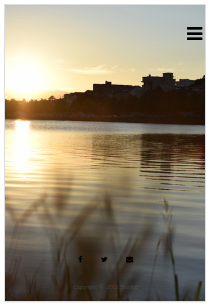
\includegraphics[width=.3\linewidth]{./img/1.png}
  \captionof{figure}{321x480}
  \label{fig:test1}
\end{minipage}%
\begin{minipage}{.5\textwidth}
  \centering
  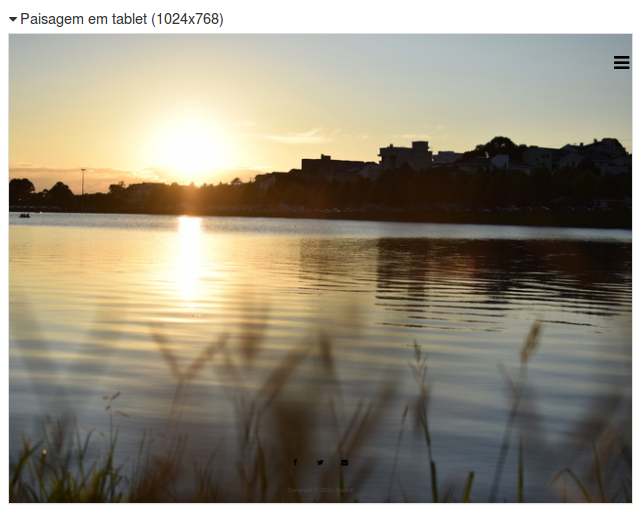
\includegraphics[width=.8\linewidth]{./img/6.png}
  \captionof{figure}{1024x768}
  \label{fig:test2}
\end{minipage}
\end{figure}
\chapter{Exigências Específicas}
	O sistema deve ser implementado contendo as funcionalidades referentes aos tópicos apresentados abaixo. Cada tópico será avaliado separadamente. Para o aluno obter nota máxima em cada tópico, ele precisa utilizar todas as estruturas listadas nos respectivos sub-tópicos. Também serão consideradas as boas práticas de programação em JavaScript, uso adequado de notações e conceitos aprendidos, organização do código e criatividade.

\section{Qualidade do código}
Estes itens foram retirado conforme combinado em sala de aula.
Style Guide
Strict mode
\subsection{Hint}
	Objetivo: mostrar a correção de apenas 5 problemas informados pelo lint ou hint.
	
Problema 1
\begin{figure}[!htb]
\setcounter{figure}{0}
\centering
\begin{minipage}{.5\textwidth}
  \centering
  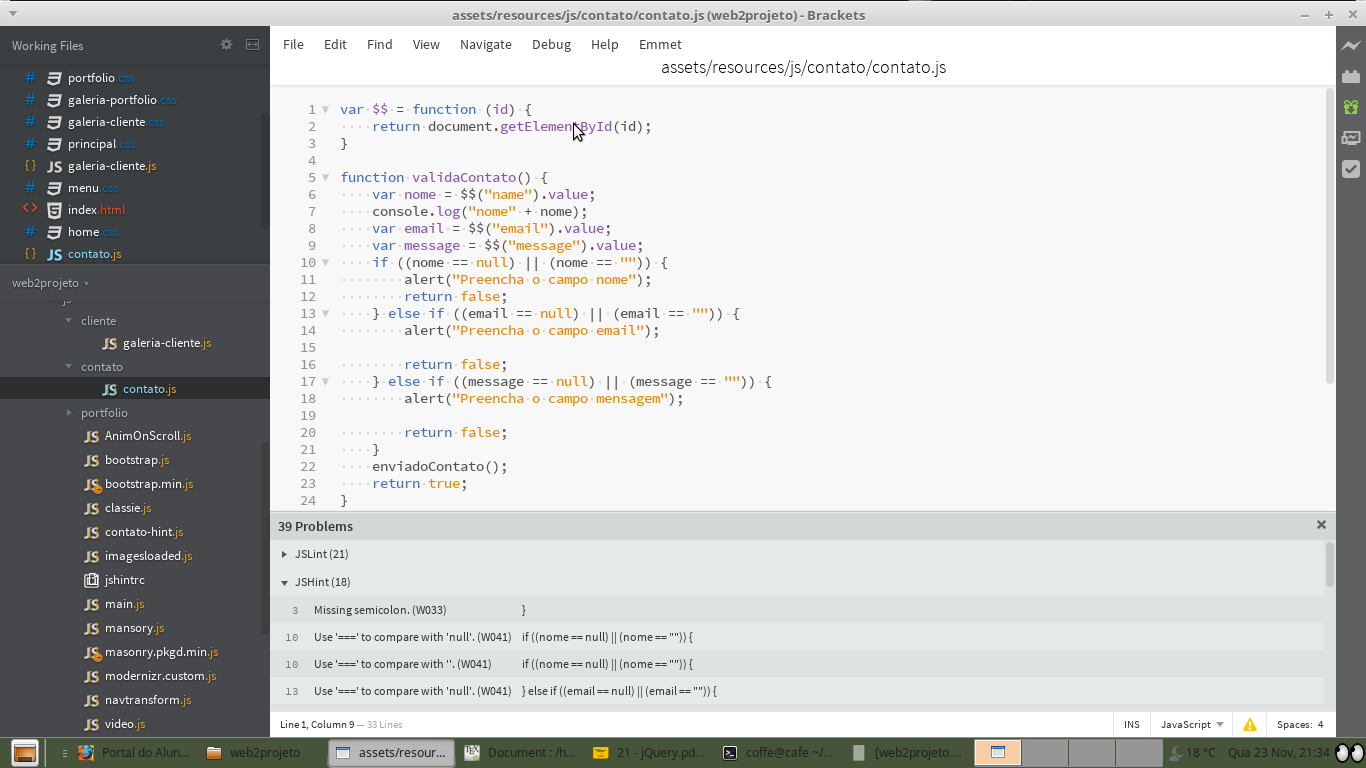
\includegraphics[width=.9\linewidth]{./img/hint1.png}
  \captionof{figure}{Problema 1}
\end{minipage}%
\begin{minipage}{.5\textwidth}
  \centering
  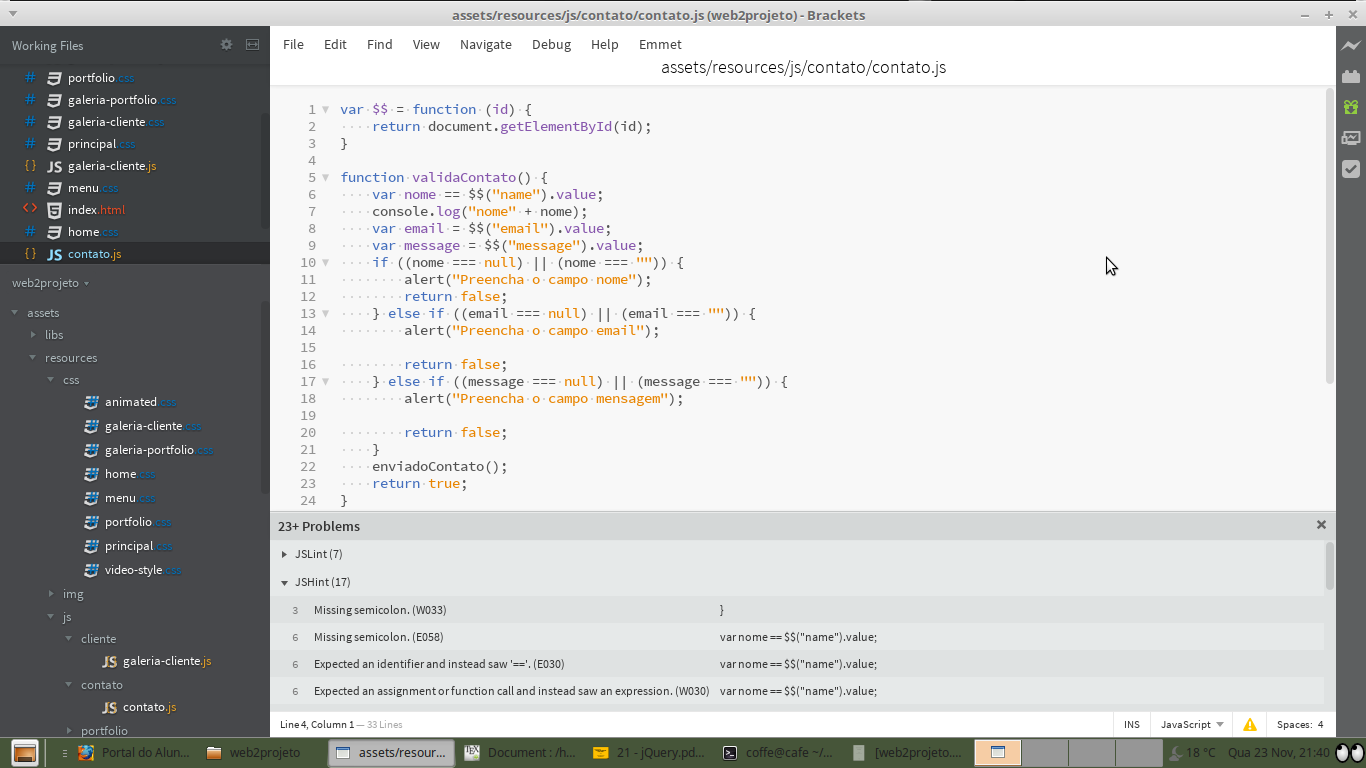
\includegraphics[width=.7\linewidth]{./img/hint1-arrumado.png}
  \captionof{figure}{Problema 1 - Correção}
\end{minipage}
\end{figure}	

Problema 2
\begin{figure}[!htb]
\setcounter{figure}{0}
\centering
\begin{minipage}{.5\textwidth}
  \centering
  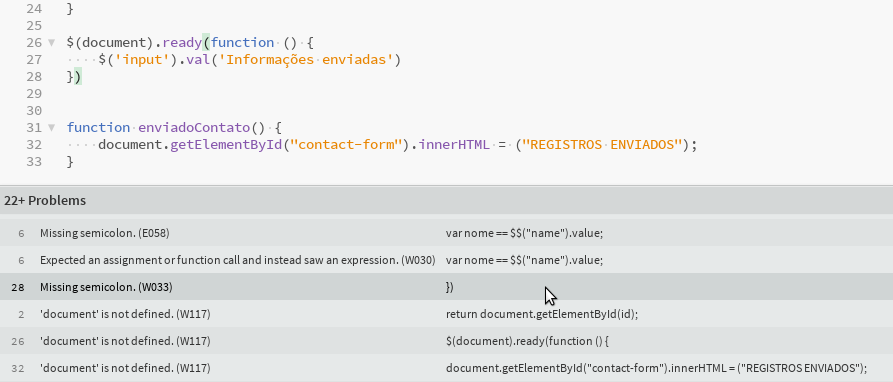
\includegraphics[width=.9\linewidth]{./img/hint2.png}
  \captionof{figure}{Problema 2}
\end{minipage}%
\begin{minipage}{.5\textwidth}
  \centering
  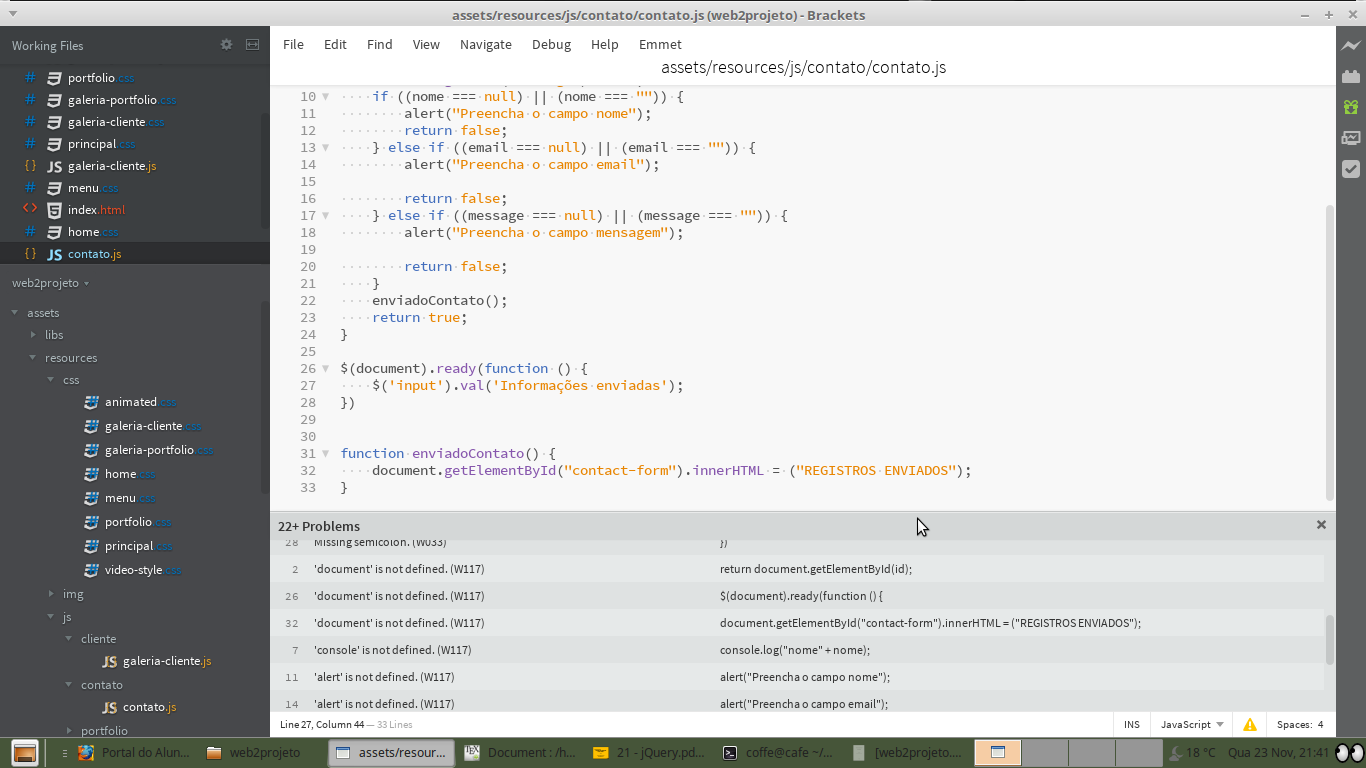
\includegraphics[width=.7\linewidth]{./img/hint2-arrumado.png}
  \captionof{figure}{Problema 2 - Correção}
\end{minipage}
\end{figure}	


Problema 3
\begin{figure}[!htb]
\setcounter{figure}{0}
\centering
\begin{minipage}{.5\textwidth}
  \centering
  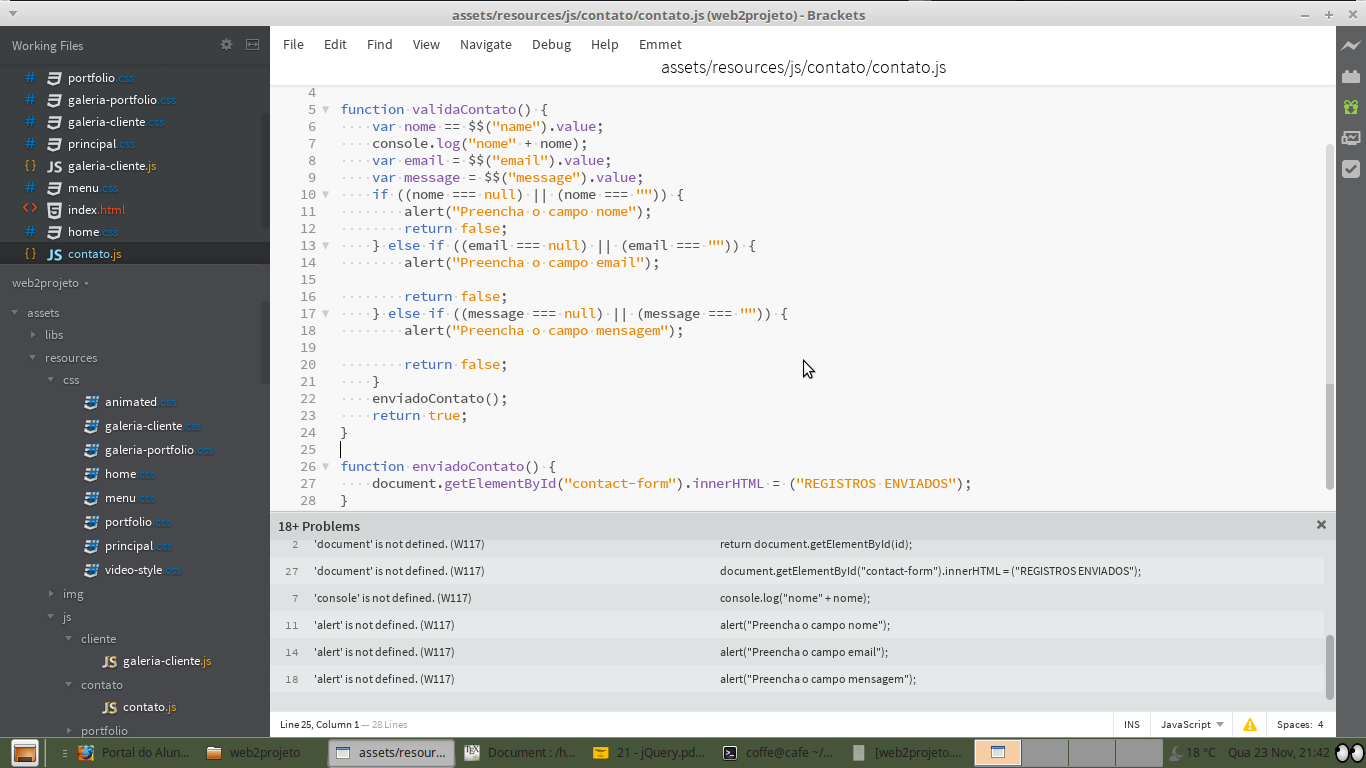
\includegraphics[width=.9\linewidth]{./img/hint3.png}
  \captionof{figure}{Problema 3}
\end{minipage}%
\begin{minipage}{.5\textwidth}
  \centering
  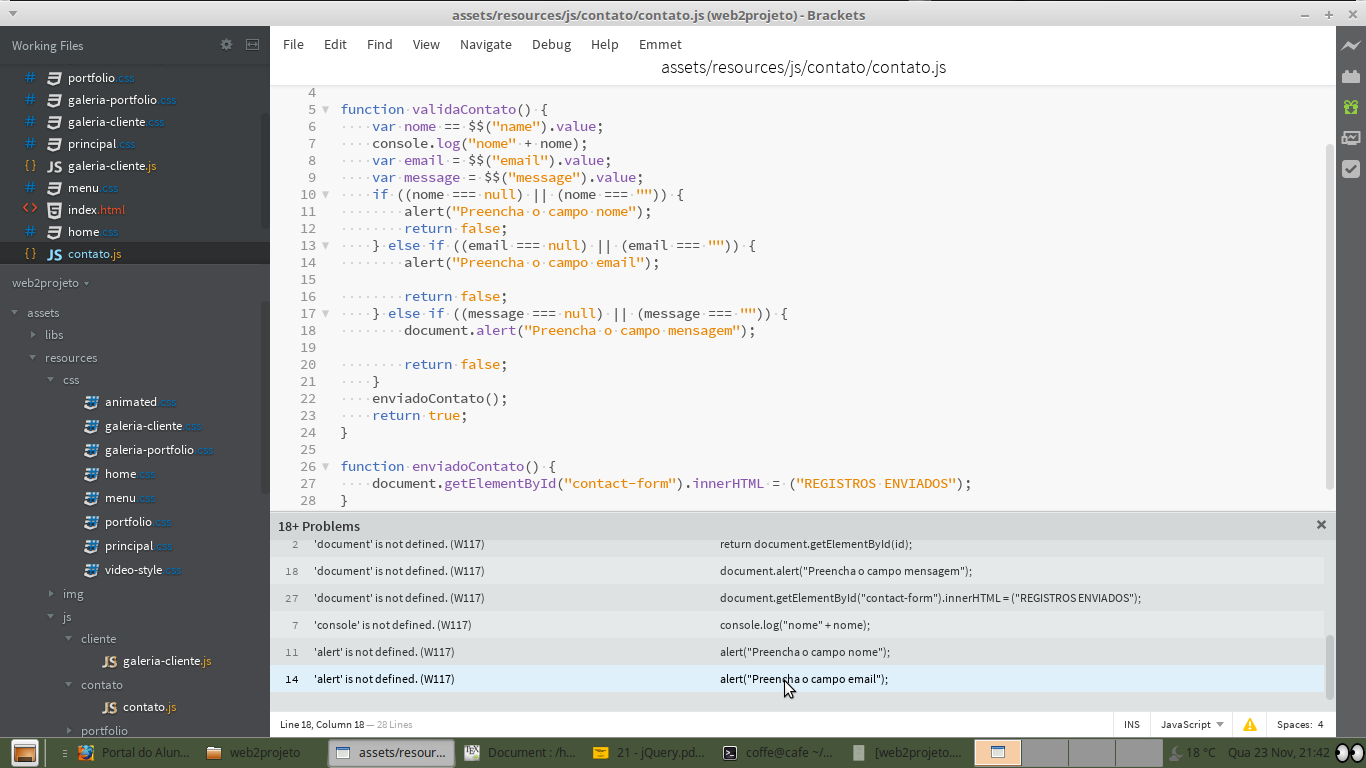
\includegraphics[width=.7\linewidth]{./img/hint3-arrumado.png}
  \captionof{figure}{Problema 3 - Correção}
\end{minipage}
\end{figure}

Problema 4
\begin{figure}[!htb]
\setcounter{figure}{0}
\centering
\begin{minipage}{.5\textwidth}
  \centering
  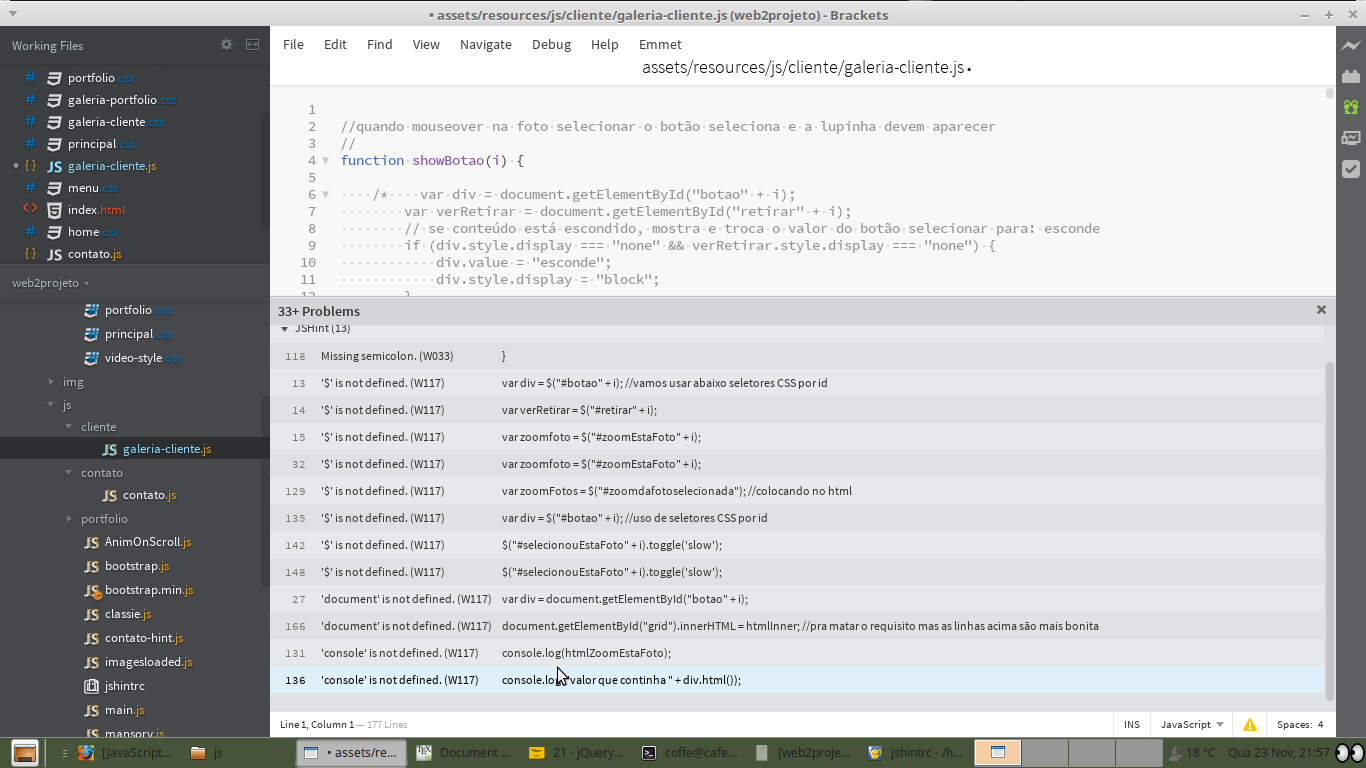
\includegraphics[width=.9\linewidth]{./img/hint4.png}
  \captionof{figure}{Problema 4}
\end{minipage}%
\begin{minipage}{.5\textwidth}
  \centering
  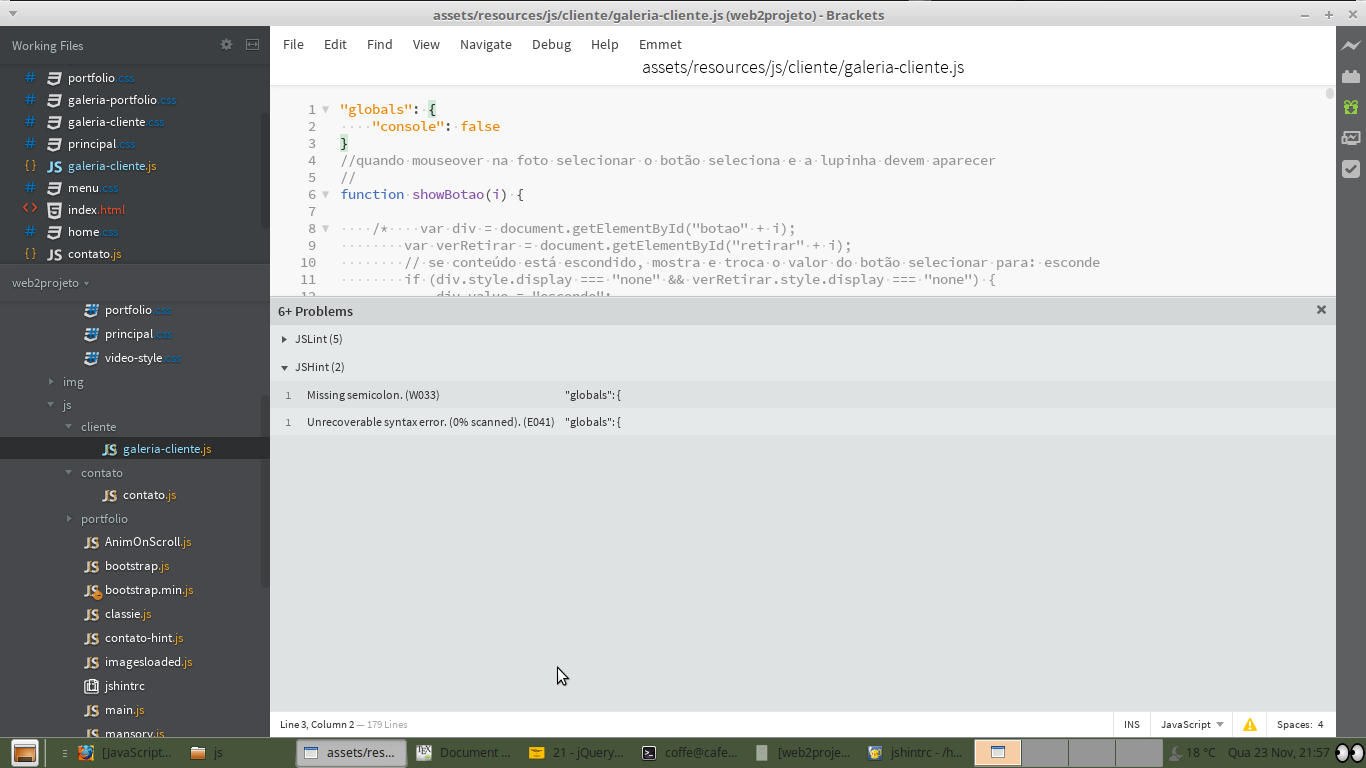
\includegraphics[width=.7\linewidth]{./img/hint4-arrumado.png}
  \captionof{figure}{Problema 4 - Correção}
\end{minipage}
\end{figure}	

\section{Caixas de Diálogo}

\subsection{prompt}

	Ver arquivo $galeria_cliente.js$
	
\begin{lstlisting}

function enviarFotosSelecionadas() {
    var confirma = confirm("Confirmar o envio das fotos?!");
    if (confirma == true) {
        var email = prompt("Por favor coloque um email para que possamos lhe comunicar sobre a entrega: ");
        //$(this).replaceWith($('<h5>' + this.innerHTML + '</h5>'));
        var fotosenviadas = { //comecamos armazenando email do cliente
            email: email,
            qtdeFotos: jsonClienteX.qtdeFotos
        };
        for (var i = 0; i < jsonClienteX.fotos.length; i++) {
            if (jsonClienteX.fotos[i].escolhido == true) {
                fotosenviadas[i] = jsonClienteX.fotos[i].arquivo; //armazenando todos os nomes dos arquivos
                console.log("enviando fotos" + i + "estava marcada no localstorage");
            }
        }
        var chaveParaAdmin = "FotosSalvasDe" + sessionStorage.getItem("logou");
        localStorage.setItem(chaveParaAdmin, JSON.stringify(fotosenviadas));
        localStorage.removeItem(sessionStorage.getItem("logou"));
        alert("Suas fotos foram enviadas Você será redirecionado para o inicio");
        deslogar();

    } else {
        return;
    }
}
\end{lstlisting}

\subsection{alert}

	No arquivo $JavaScript$ chamado $contato.js$ criamos uma função com nome $validaContato()$ conforme segue abaixo para melhor visualização:
	
\begin{lstlisting}
function validaContato() {
    var nome = $$("name").value;
    console.log("nome" + nome);
    var email = $$("email").value;
    var message = $$("message").value;
    if ((nome == null) || (nome == "")) {
        alert("Preencha o campo nome");
        return false;
    } else if ((email == null) || (email == "")) {
        alert("Preencha o campo email");
        return false;
    } else if ((message == null) || (message == "")) {
        alert("Preencha o campo mensagem");
        return false;
    }
    return true;
}
\end{lstlisting}
	Esta função está relacionada a validação dos campos do formulário. E dentro dela utilizamos $alert$ para enviar uma mensagem ao visitante da página.

\subsection{confirm}
	No arquivo $JavaScript$ chamado $galeria$\_$cliente.js$.
	Criamos uma função com nome $enviarFotosSelecionadas()$ conforme segue abaixo para melhor visualização:
	
\begin{lstlisting}
function enviarFotosSelecionadas() {
    var confirma = confirm("Confirmar o envio das fotos?!");
    if (confirma == true) {
        var email = prompt("Por favor coloque um email para que possamos lhe comunicar sobre a entrega: ");
        var fotosenviadas = { //comecamos armazenando email do cliente
            email: email
        };
        for (var i = 0; i < jsonClienteX.fotos.length; i++) {
            if (jsonClienteX.fotos[i].escolhido == true) {
                fotosenviadas[i] = jsonClienteX.fotos[i].arquivo; //armazenando todos os nomes dos arquivos
                console.log("enviando fotos" + i + "estava marcada no localstorage");
            }
        }
        var chaveParaAdmin = "FotosSalvasDe" + sessionStorage.getItem("logou"); //id do cliente sessionStorage.getItem("logou")
       
        localStorage.setItem(chaveParaAdmin, JSON.stringify(fotosenviadas));

        localStorage.removeItem(sessionStorage.getItem("logou"));

        alert("Suas fotos foram enviadas Você será redirecionado para o inicio");
        deslogar();

    } else {
        return;
    }
}
\end{lstlisting}
	Observe que na segunda linha da função temos o solicitado.

\section{Funções}
\subsection{Função anônima com argumento}
	No arquivo $JavaScript$ chamado $login.js$ criamos uma função anônima que receberá um argumento $i$ conforme segue abaixo para melhor visualização:
	
\begin{lstlisting}
var naoLogou = function (i) {
    var logou;
    if (i == 23) {
        sessionStorage.setItem("logou", "1267");
    }
}
\end{lstlisting}

\subsection{Função anônima sem argumento}
	Verificar o arquivo $admin.js$ 
\begin{lstlisting}
$(function () {
    var setContentHeight = function () {
        // reseta altura
        $RIGHT_COL.css('min-height', $(window).height());

        var bodyHeight = $BODY.height(),
            leftColHeight = $LEFT_COL.eq(1).height() + $SIDEBAR_FOOTER.height(),
            contentHeight = bodyHeight < leftColHeight ? leftColHeight : bodyHeight;

        // configura página de conteúdo
        contentHeight -= $NAV_MENU.height() + $FOOTER.height();

        $RIGHT_COL.css('min-height', contentHeight);
    };

    $SIDEBAR_MENU.find('a').on('click', function (ev) {
        var $li = $(this).parent();

        if ($li.is('.active')) {
            $li.removeClass('active');
            $('ul:first', $li).slideUp(function () {
                setContentHeight();
            });
        } else {
            // previse que o menu seja fechado estando nos itens de menus filhos.
            if (!$li.parent().is('.child_menu')) {
                $SIDEBAR_MENU.find('li').removeClass('active');
                $SIDEBAR_MENU.find('li ul').slideUp();
            }

            $li.addClass('active');

            $('ul:first', $li).slideDown(function () {
                setContentHeight();
            });
        }
    });

    // menu responsivo
    $MENU_TOGGLE.on('click', function () {
        if ($BODY.hasClass('nav-md')) {
            $BODY.removeClass('nav-md').addClass('nav-sm');
            $LEFT_COL.removeClass('scroll-view').removeAttr('style');

            if ($SIDEBAR_MENU.find('li').hasClass('active')) {
                $SIDEBAR_MENU.find('li.active').addClass('active-sm').removeClass('active');
            }
        } else {
            $BODY.removeClass('nav-sm').addClass('nav-md');

            if ($SIDEBAR_MENU.find('li').hasClass('active-sm')) {
                $SIDEBAR_MENU.find('li.active-sm').addClass('active').removeClass('active-sm');
            }
        }
        setContentHeight();
    });

    // vefica se o meno esta ativo ou não e qual pagina está
    $SIDEBAR_MENU.find('a[href="' + URL + '"]').parent('li').addClass('current-page');

    $SIDEBAR_MENU.find('a').filter(function () {
        return this.href == URL;
    }).parent('li').addClass('current-page').parents('ul').slideDown(function () {
        setContentHeight();
    }).parent().addClass('active');

    // organiza a diminsão do conteúdo.
    $(window).smartresize(function () {
        setContentHeight();
    });

});	
\end{lstlisting}	
\subsection{Função anônima auto-executável}
	Ver no arquivo $contato.js$

\begin{lstlisting}
(function () { 
    tagDesnegrito();
});

\end{lstlisting}

\subsection{Função com nome}

	No arquivo $JavaScript$ chamado $contato.js$ criamos uma função com nome $validaContato()$ conforme segue abaixo para melhor visualização:
\begin{lstlisting}
function validaContato() {
    var nome = $$("name").value;
    console.log("nome" + nome);
    var email = $$("email").value;
    var message = $$("message").value;
    if ((nome == null) || (nome == "")) {
        alert("Preencha o campo nome");
        return false;
    } else if ((email == null) || (email == "")) {
        alert("Preencha o campo email");
        return false;
    } else if ((message == null) || (message == "")) {
        alert("Preencha o campo mensagem");
        return false;
    }
    return true;
}
\end{lstlisting}
	Esta função está relacionada a validação dos campos do formulário.

\subsection{Função aninhada/interna}

	Esta função está relacionada a construção de uma $grid$ de fotos do cliente, uma galeria de fotos. A função  $exibirFotosAoIniciar()$ é chamada quando a página é carregada, ela sempre irá  verificar antes se o cliente está logado, pois do contrário não poderemos mostrar ao visitante as fotos, isto é a galeria não será carregada. 
	
\begin{lstlisting}
function exibirFotosAoIniciar() {
    var logou = verSeLogado();
    if (!logou) {
        return;
    }
    var htmlInner = "";
    for (var i = 0; i < jsonClienteX.fotos.length; i++) {
        htmlInner += '<li>\n<div class = "caption img-wrapper" onmouseover="showBotao(' + i + ');" onmouseout="escondeBotaoSelecionar(' + i + ');" style="position:relative;">\n<img src="';
        htmlInner += jsonClienteX.pasta + jsonClienteX.fotos[i].arquivo + jsonClienteX.extensao;
        htmlInner += '">\n<div class="selecionouEstaFoto" id="selecionouEstaFoto' + i + '" style="display:none"><span class="glyphicon glyphicon-ok"> </span></div>\n <div class="zoomEstaFoto" id="zoomEstaFoto' + i + '" style="display:none"><a href="#" data-toggle="modal" data-target="#myModal" onclick=zoomFotoLinha(' + i + '); <span class="glyphicon glyphicon-zoom-in"> </span></a></div >\n<button id="botao' + i + '" style="display:none" class="btn btn-success" onclick="alternarEscolhaDaFoto(' + i + ');">Selecionar</button></div>\n</li>';
    }
    document.getElementById("grid").innerHTML = htmlInner;
}
\end{lstlisting}


\subsection{Passagem de uma função como parâmetro}
	Para este item consideremos no arquivo $javascript$ da galeria do cliente a função $alternarEscolhaDaFoto(i)$, dentro dela veja a linha $4$.	
	
\begin{lstlisting}	
function alternarEscolhaDaFoto(i) {
    console.log("valor que continha " + div.html());
    if (div.html() == "Selecionar") {
        selecionaOuRetiraFoto(i, selecionarFoto);
    } else {
        selecionaOuRetiraFoto(i, deselecionarFoto);
    }
    //salvando cada as fotos selecionada
    var chaveCliente = sessionStorage.getItem("logou");
    localStorage.setItem(chaveCliente, JSON.stringify(jsonClienteX));
}
var selecionaOuRetiraFoto = function (i, executar) {
    executar(i);
}

\end{lstlisting}
	Na linha $4$ temos a função solicitada que recebe por parâmetro a função $selecionarFoto$ dentro dela aplica o prâmetro $i$ também recebido. Abaixo temos o código da função $selecionarFoto(i)$.
	
\begin{lstlisting}
function selecionarFoto(i) {
    var div = $("#botao" + i); //uso de seletores CSS por id
    div.toggle('slow').toggle('slow');
    div.html("Retirar");
    jsonClienteX.fotos[i].escolhido = true;
    div.removeClass('btn-success').addClass('btn-warning');
    $("#selecionouEstaFoto" + i).toggle('slow');
    div.fadeOut(500);
    jsonClienteX.qtdeFotos++;
}

function deselecionarFoto(i) {
    var div = $("#botao" + i); //uso de seletores CSS por id
    div.html("Selecionar");
    jsonClienteX.fotos[i].escolhido = false;
    div.removeClass('btn-warning').addClass('btn-success');
    $("#selecionouEstaFoto" + i).toggle('slow');
    jsonClienteX.qtdeFotos--;
}	
	\end{lstlisting}

\section{Eventos}

\subsection{Evento de carregamento do documento}
	Para este item verificar no arquivo $cliente.html$ as seguintes linhas:
	\begin{lstlisting}
	    <script>
        $(document).ready(function () {
            exibirFotosAoIniciar();
            $(window).scroll(function () {
                set = $(document).scrollTop() + "px";
                jQuery('#float-banner').animate({
                    top: set
                }, {
                    duration: 1000,
                    queue: false
                });
            });
            console.log("pronto carregada a página! Vamos trabalhar js ");
            new AnimOnScroll(document.getElementById('grid'), {
                minDuration: 0.4,
                maxDuration: 0.7,
                viewportFactor: 0.2
            });
        });
    </script>
	\end{lstlisting}
\subsection{Evento de movimento do mouse}
	No arquivo $about.html$ temos:
\begin{lstlisting}
	<p onmouseover="tagNegrito()" onmouseout="tagDesnegrito()">
\end{lstlisting}
\subsection{Evento de teclado}
 Objetivo:  - usar charCode ou KeyCode.
 	Este item foi retirado conforme combinado em sala de aula.
 
\subsection{Eventos de formulário}
	Objetivo: onfocus e onblur. Verificar arquivo $contato.js$
	
 \begin{lstlisting}
  window.onload = function() {
  var input_name = document.forms[0].name;
  var input_email = document.forms[0].email;
  var input_msg = document.forms[0].message;

  input_name.addEventListener('blur', function() {
    if (input_name.value == "")
      input_name.value = "Você esqueceu de preencher-me";
  });

  input_email.addEventListener('blur', function() {
    if (input_email.value == "")
      input_email.value = "Você esqueceu de preencher-me";
  });

   input_msg.addEventListener('blur', function() {
    if (input_msg.value == "")
      input_msg.value = "Você esqueceu de preencher-me";
  });

  input_name.addEventListener('focus', function() {
    input_name.style.color = '#fff';
    input_name.style.background = '#0080ff';

    input_email.style.color = '#000';
    input_email.style.background = '#fff';

    input_msg.style.color = '#000';
    input_msg.style.background = '#fff';
  });

  input_email.addEventListener('focus', function() {
    input_name.style.color = '#000';
    input_name.style.background = '#fff';

    input_email.style.color = '#fff';
    input_email.style.background = '#0080ff';

    input_msg.style.color = '#000';
    input_msg.style.background = '#fff';
  });

  input_msg.addEventListener('focus', function() {
    input_msg.style.color = '#fff';
    input_msg.style.background = '#0080ff';

    input_email.style.color = '#000';
    input_email.style.background = '#fff';

    input_name.style.color = '#000';
    input_name.style.background = '#fff';
  });
 \end{lstlisting}
\subsection{objeto event}
Obejtivo: Imprimir alguma propriedade do objeto event recebido como parâmetro. Ao começar a preencher o formulário da página $contato.html$ estaremos fazendo uso do $event$ para reescrever próximo a tag $<span>$ tudo o que foi digitado no campo.

 \begin{lstlisting}
function validarString(campo, event) {
    var id = event.target.id;
    if (campo == "nome") {
        //trate nome
        validarNome(id, event.target.value);
    } else if (campo == "email") {
        //trate nome
        validarEmail(id, event.target.value);
    } else if (campo == "mensagem") {
        //trate nome
        validarMensage(id, event.target.value);
    }
}

function validarNome(id, txt) {
    var mensage = $('#lb' + id);
    if (txt.length > 30) {
        mensage.html(txt.substr(0, 25) + " ... " + txt.substr(txt.length - 4, 4));
    } else {
        mensage.html(txt);
    }
}

function validarEmail(id, txt) {
    var mensage = $('#lb' + id);
    if (txt.length > 18) {
        mensage.html(txt.substr(0, 14) + " ... " + txt.substr(txt.length - 4, 4));
    } else {
        mensage.html(txt);
    }
}

function validarMensage(id, txt) {
    var mensage = $('#lb' + id);
    if (txt.length > 30) {
        mensage.html(txt.substr(0, 24) + " ... " + txt.substr(txt.length - 4, 4));
    } else {
        mensage.html(txt);
    }
}
\end{lstlisting}

\subsection{Propagação de eventos no modelo bolha}
 	Este item foi retirado conforme combinado em sala de aula.
\section{Acesso aos elementos DOM do HTML }
\subsection{Via acesso direto}

 Pelo id do elemento HTML utilizamos a função $loginCliente()$ no arquivo $login.js$
 \begin{lstlisting}
 function loginCliente() {
    //var email = document.getElementById("email").value;
    var email = window.email.value;
    var password = document.getElementById("password").value;
    console.log("entrou aqui" + email + " e " + password);
    if (email == "teste@gmail.com" && password == "projeto$$") {
        naoLogou(23);
        alert("Obrigada por fazer login voce sera redirecionado (a).");
        window.location = "cliente.html";
        return false;
    } else {
        tentativas--;
        alert("Voce tem: " + tentativas + " tentativas;");
        if (tentativas == 0) {
            document.getElementById("email").disabled = true;
            document.getElementById("password").disabled = true;
            document.getElementById("submit").disabled = true;
            return false;
        }
    }
}
 \end{lstlisting}

\subsection{Via getElementByID()}
	Ver arquivo $contato.html$ a função $enviadoContato()$, conforme código abaixo:
	
\begin{lstlisting}
function enviadoContato() {
    document.getElementById("contact-form").innerHTML = ("REGISTROS ENVIADOS");
}
\end{lstlisting}

\subsection{Via getElementsByName()}

	Considerar o arquivo $admin.js$
\begin{lstlisting}
	function insereSelect() {
    console.log("quququq");
    var x = document.getElementsByTagName('select')[0].length;
    document.getElementsByName("selecionandofotos")[0].innerHTML = "Quantide de clientes: " + x;
}
\end{lstlisting}

\subsection{Via getElementsByTagName()}
	Considerar o arquivo $admin.js$
\begin{lstlisting}
	function insereSelect() {
    console.log("quququq");
    var x = document.getElementsByTagName('select')[0].length;
    document.getElementsByName("selecionandofotos")[0].innerHTML = "Quantide de clientes: " + x;
}
\end{lstlisting}


\subsection{Via seletores CSS}
	O botão enviar da página $cliente.html$ é um $banner$ que fica seguinto a ação de rolar a página. Para isto adicionamos no arquivo $cliente.html$ algumas linhas, dentre elas temos esta:
		\begin{lstlisting}	
	jQuery('#float-banner').animate({
		\end{lstlisting}
		Este $selector$ irá se referir ao $id="float-banner"$, que no arquivo $HTML$ está representado com as linhas abaixo:
\begin{lstlisting}
<div id="float-banner">
     <a class="btn btn-default btn-lg btn-sm" href="#" role="button" onclick="return enviarFotosSelecionadas()"><span class="glyphicon glyphicon-send"></span> ENVIAR </a>
</div>
\end{lstlisting}

	Abaixo seguem todas as linhas da função do $JQuery$ $(document).ready(function$ $()$ que utilizamos por ser parecida com o $window.onload$, exceto que no $JQuery$ não precisamos esperar o carregamento de imagens como no $window.onload$ (nesta página isto será útil pois temos muitas fotos).
	
		\begin{lstlisting}
	    <script>
        $(document).ready(function () {
            exibirFotosAoIniciar();
            $(window).scroll(function () {
                set = $(document).scrollTop() + "px";
                jQuery('#float-banner').animate({
                    top: set
                }, {
                    duration: 1000,
                    queue: false
                });
            });
            console.log("pronto carregada a página! Vamos trabalhar js ");
            new AnimOnScroll(document.getElementById('grid'), {
                minDuration: 0.4,
                maxDuration: 0.7,
                viewportFactor: 0.2
            });
        });
    </script>
	\end{lstlisting} 
  
  
\section{Tratadores de Evento}
\subsection{Evento inline}
Objetivo: especificar o tratador de evento inline. Tratador de eventos inline - onmouseover, onmouseout ou onclick. Neste item escolhemos utilizar $onclick$

$onclick$ - Ver no arquivo $galeria$\_$cliente.js$ a seguinte linha:

\begin{lstlisting}
<button id="botao' + i + '" style="display:none" class="btn btn-success" onclick="alternarEscolhaDaFoto(' + i + ');">Selecionar</button>
\end{lstlisting}

	Esta linha irá criar o botão Selecionar. Nela é mostrado uma ação para $onclick$ que chama a função $alternarEscolhaDaFoto(i)$ - I $i$ é um parâmetro referente a foto que estará sendo mostrada.
	

\subsection{Modo tradicional}
Objetivo: especificar o tratador de evento no carregamento da página HTML no modo tradicional.

Verificar arquivo $contato.js$
	
 \begin{lstlisting}
  window.onload = function() {
    var input_name = document.forms[0].name;
    var input_email = document.forms[0].email;
    var input_msg = document.forms[0].mensage;
...
  });
 \end{lstlisting}



\subsection{addEventListener}
 Objetivo: especificar o tratador de evento no carregamento da página HTML com a função addEventListener.
	Verificar arquivo $contato.js$
 \begin{lstlisting}
window.onload = function () {
    var input_name = document.forms[0].name;
    var input_email = document.forms[0].email;
    var input_msg = document.forms[0].mensage;

    input_name.addEventListener('blur', function (e) {
        if (input_name.value == "")
            $("#lbname").html("Você esqueceu de preencher nome");
    });

    input_email.addEventListener('blur', function () {
        if (input_email.value == "")
            $("#lbemail").html("Você esqueceu de preencher email");
    });

    input_msg.addEventListener('blur', function () {
        if (input_msg.value == "")
            $("#lbmensage").html("Você esqueceu de preencher a mensagem");
    });

    input_name.addEventListener('focus', function () {
        input_name.style.color = '#fff';
        input_name.style.background = '#0080ff';

        input_email.style.color = '#000';
        input_email.style.background = '#fff';

        input_msg.style.color = '#000';
        input_msg.style.background = '#fff';
    });

    input_email.addEventListener('focus', function () {
        input_name.style.color = '#000';
        input_name.style.background = '#fff';

        input_email.style.color = '#fff';
        input_email.style.background = '#0080ff';

        input_msg.style.color = '#000';
        input_msg.style.background = '#fff';
    });

    input_msg.addEventListener('focus', function () {
        input_msg.style.color = '#fff';
        input_msg.style.background = '#0080ff';

        input_email.style.color = '#000';
        input_email.style.background = '#fff';

        input_name.style.color = '#000';
        input_name.style.background = '#fff';
    });
}
 \end{lstlisting} 
 
 
\subsection{Operador this}
 Objetivo: usar o operador this em funções tratadoras de eventos.
 
 	Este item foi retirado conforme combinado em sala de aula.


\section{Formulário}
	Foi criado a página $contato.html$. Nesta página temos um formulário com $3$ campos de preenchimento obrigatórios.
	
\subsection{Validação}
	Objetivo: validação de formulário com onsubmit usando os métodos tradicionais.
	
	Para cumprir o objetivo o formulário $contato.html$ faz uso da seguinte maneira:
\begin{lstlisting}
<form id="contact-form" class="validate-form" method="post" onsubmit="return validaContato()">
\end{lstlisting}

	O arquivo $JavaScript$ chamado $contato.js$ contém a função com nome $validaContato()$:
\begin{lstlisting}
function validaContato() {
    var nome = $$("name").value;
    console.log("nome" + nome);
    var email = $$("email").value;
    var message = $$("message").value;
    if ((nome == null) || (nome == "")) {
        alert("Preencha o campo nome");
        return false;
    } else if ((email == null) || (email == "")) {
        alert("Preencha o campo email");

        return false;
    } else if ((message == null) || (message == "")) {
        alert("Preencha o campo mensagem");

        return false;
    }
    enviadoContato();
    return true;
}
\end{lstlisting}
	

\subsection{Propriedade Value}
	Objetivo: ler e escrever em elementos $input$ com a propriedade $value$
	
\begin{lstlisting}
$(document).ready(function () {
    $('input').val('Informacoes enviadas')
})
\end{lstlisting}


\subsection{innerHtml}
	Objetivo: alterar o conteúdo de elementos $div$ ou $p$com a propriedade $innerHTML$
	
	Para este item escolhemos alterar o elemento $div$ do formulário de $contatos$ pois assim que o visitante enviar uma mensagem de contato a estrutura do formulário será substituída por uma frase, conforme código abaixo, definido pela função.

\begin{lstlisting}
function enviadoContato() {
    document.getElementById("contact-form").innerHTML = ("REGISTROS ENVIADOS");
}
\end{lstlisting}


\subsection{checkbox, radio ou select}
	Utilizamos um select no arquivo $admin.html$. Este select é montado no arquivo $javascript$ $admin_clientes.js$ e o objetivo deste select é monstrar ao administrador todos os clientes que possuem fotos para serem tratadas/editadas. Estas fotos foram selecionadas pelo cliente anteriormente.
\begin{lstlisting}	
	function verFotosSelecionadas() {
    var variaveleSelect = $('select');
    for (chave in localStorage) {
        if (chave.indexOf("FotosSalvasDe") >= 0) { //esta é a chave de um cliente que enviou fotos
            console.log("dentro do if");
            var chaveDoCliente = chave.replace("FotosSalvasDe", "");
            console.log("dentro do if chaveDoCliente" + chaveDoCliente);
            //botar no select
            variaveleSelect.append('<option val="' + chaveDoCliente + '">' + chaveDoCliente + '</option>');
        }
    }
    console.log("quantidade de clientes");
    var x = document.getElementsByTagName('select')[0].length;
    document.getElementsByName("selecionandofotos")[0].innerHTML = "Quantide de clientes: " + x;
}

\end{lstlisting}
\subsection{Acesso via hierarquia}
	Acesso aos elementos de um formulário via hierarquia (caminho) de objetos, ou seja, array forms e elements.
 Verificar arquivo $contato.js$
	
 \begin{lstlisting}
  window.onload = function() {
  var input_name = document.forms[0].name;
  var input_email = document.forms[0].email;
  var input_msg = document.forms[0].message;

  
 \end{lstlisting}	
	

\section{Objetos Nativos }
\subsection{Manipulação de array}
	Usar métodos para manipulação de array - Para este item observar o Array fotos dentro do objeto $jsonClientX$

\begin{lstlisting}	
	var jsonClienteX = {
    pasta: "assets/resources/img/clients/cliente/",
    extensao: ".jpg",
    qtdeFotos: 0,
    fotos: [
        {
            arquivo: '2',
            escolhido: false
        },
        {
            arquivo: '20',
            escolhido: false
        },
	],
}
\end{lstlisting}

\subsection{Manipulação de string}
Usar métodos para manipulação de string. Para este item verificar no arquivo $admin_clientes.js$ a função $verFotosSelecionadas()$, utilizamos $indexOf$ (linha $4$):
\begin{lstlisting}	
function verFotosSelecionadas() {
    var variaveleSelect = $('select');
    for (chave in localStorage) {
        if (chave.indexOf("FotosSalvasDe") >= 0) { //esta é a chave de um cliente que enviou fotos
            console.log("dentro do if");
            var chaveDoCliente = chave.replace("FotosSalvasDe", "");
            console.log("dentro do if chaveDoCliente" + chaveDoCliente);
            //botar no select
            variaveleSelect.append('<option val="' + chaveDoCliente + '">' + chaveDoCliente + '</option>');
        }
    }
    console.log("quantidade de clientes");
    var x = document.getElementsByTagName('select')[0].length;
    document.getElementsByName("selecionandofotos")[0].innerHTML = "Quantide de clientes: " + x;
}
\end{lstlisting}
\section{Objetos}
\subsection{Criar objeto}
	Criar objeto usando função construtora ou notação literal
\begin{lstlisting}	
	var jsonClienteX = {
    pasta: "assets/resources/img/clients/cliente/",
    extensao: ".jpg",
    qtdeFotos: 0,
    fotos: [
        {
            arquivo: '2',
            escolhido: false
        },
        {
            arquivo: '20',
            escolhido: false
        },
        {
            arquivo: '3',
            escolhido: false
        },
        {
            arquivo: '4',
            escolhido: false
        },
        {
            arquivo: '5',
            escolhido: false
        },
        {
            arquivo: '20',
            escolhido: false
        },
        {
            arquivo: '6',
            escolhido: false
        },
        {
            arquivo: '8',
            escolhido: false
        },
        {
            arquivo: '9',
            escolhido: false
        },
        {
            arquivo: '10',
            escolhido: false
        },
        {
            arquivo: '11',
            escolhido: false
        },
        {
            arquivo: '12',
            escolhido: false
        },
        {
            arquivo: '13',
            escolhido: false
        },
        {
            arquivo: '14',
            escolhido: false
        },
        {
            arquivo: '15',
            escolhido: false
        },
        {
            arquivo: '16',
            escolhido: false
        },
        {
            arquivo: '17',
            escolhido: false
        },
        {
            arquivo: '18',
            escolhido: false
        },
        {
            arquivo: '19',
            escolhido: false
        },
	],
}
\end{lstlisting}

\subsection{Herança}
Usar herança prototipal.
 	Este item foi retirado conforme combinado em sala de aula.

\section{jQuery}
\subsection{Seletores CSS}

	Uso de seletores CSS - id, classe e tag. Os subitem abaixo nos mostram como foram utilizados os seletores solicitados.
	
\subsubsection{id}
	Verificar a linha $6$ abaixo:
		\begin{lstlisting}
	    <script>
        $(document).ready(function () {
            exibirFotosAoIniciar();
            $(window).scroll(function () {
                set = $(document).scrollTop() + "px";
                jQuery('#float-banner').animate({
                    top: set
                }, {
                    duration: 1000,
                    queue: false
                });
            });
            console.log("pronto carregada a página! Vamos trabalhar js ");
            new AnimOnScroll(document.getElementById('grid'), {
                minDuration: 0.4,
                maxDuration: 0.7,
                viewportFactor: 0.2
            });
        });
    </script>
	\end{lstlisting}

	Observar também abaixo que na linha 2 do arquivo $galeria$\_$cliente.js$ temos o uso de seletor $CSS$ por $id$.
	
\begin{lstlisting}
function deselecionarFoto(i) {
    var div = $("#botao" + i); //uso de seletores CSS por id
    div.html("Selecionar");
    jsonClienteX.fotos[i].escolhido = false;
    div.removeClass('btn-warning').addClass('btn-success');
    $("#selecionouEstaFoto" + i).toggle('slow');
}
\end{lstlisting}

\subsubsection{classe}
	Ver linha $6$.
\begin{lstlisting}
function selecionarFoto(i) {
    var div = $("#botao" + i); //uso de seletores CSS por id
    div.toggle('slow').toggle('slow');
    div.html("Retirar");
    jsonClienteX.fotos[i].escolhido = true;
    div.removeClass('btn-success').addClass('btn-warning');
    $("#selecionouEstaFoto" + i).toggle('slow');
    div.fadeOut(500);
}
\end{lstlisting}

\subsubsection{tag}
	Ver no arquivo $contato.js$ a função faz a troca de cor da letra das tags $<p>$.
\begin{lstlisting}
	function tagNegrito() {
    $("p").css("color", "black");
}


function tagDesnegrito() {
    $("p").css("color", "gray");

}

(function () { //função auto-executável
    tagDesnegrito();
    //se houver algum css negrito remover
});

\end{lstlisting}
\subsection{Seletores hierarquicos}
Uso de seletores hierarquicos - ancestral/descendente, pai/filho, anterior/proximo.
 	Este item foi retirado conforme combinado em sala de aula.

\subsection{Efeitos fade ou slide}

	Efeito utilizado $fadeout$.
	Observe na linha $8$ da função $selecionarFoto(i)$ do arquivo $galeria$\_$cliente.js$.
	
\begin{lstlisting}	
function selecionarFoto(i) {
    var div = $("#botao" + i); //uso de seletores CSS por id
    div.toggle('slow').toggle('slow');
    div.html("Retirar");
    jsonClienteX.fotos[i].escolhido = true;
    div.removeClass('btn-success').addClass('btn-warning');
    $("#selecionouEstaFoto" + i).toggle('slow');
    div.fadeOut(500);
}
\end{lstlisting}

\subsection{Tratador de algum evento}
Espeficar o tratador de algum evento via jQuery. Escolhemos mostrar o $jQuery$ $mouseover()$ $Method$ na id $\#mouseover$ do arquivo $contato.html$.
\begin{lstlisting}		
    <script>
        $(document).ready(function () {
            $("#mouseover").mouseover(function () {
                $("#mouseover").css("background-color", "white");
                $("#mouseover").css("color", "black");
            });
            $("#mouseover").mouseout(function () {
                $("#mouseover").css("background-color", "#f2f2f2");
            });
        });
    </script>
\end{lstlisting}



\subsection{Manipulação CSS}
	Objetivo: manipulação do CSS via função $css()$ e $addClass()$/$removeClass()$

	Utilizamos $addClass$ e $removeClass$ na função $alternarEscolhaDaFoto(i)$ do arquivo $galeria-cliente.js$. 
	Descrição da função: quando um cliente realizar a seleção de uma foto o botão irá mudar de cor, ficando disponível a opção para desmarcar a foto que acabou de ser selecionada, na função, veja a linha $8$. O inverso irá acontecer quando o cliente desmarcar a foto que havia sido selecionada, linha $13$.
	

\begin{lstlisting}
function alternarEscolhaDaFoto(i) {
    var div = $("#botao" + i); //uso de seletores CSS por id
    console.log("valor que continha " + div.html());
    if (div.html() == "Selecionar") {
        selecionaOuRetiraFoto(i, selecionarFoto); //passagem de uma função por parâmetro
    } else {
        selecionaOuRetiraFoto(i, deselecionarFoto);
    }
    //salvando cada as fotos selecionada
    var chaveCliente = sessionStorage.getItem("logou");

    localStorage.setItem(chaveCliente, JSON.stringify(jsonClienteX));
}
\end{lstlisting}

\subsection{Manipulação do conteúdo}
	Objetivo: manipulação do conteúdo de um $input$ e $div$ usando $jQuery$.

\section{Web Storage } 
	Abaixo todos os subitens solicitados.
\subsection{LocalStorage}
	Fazemos uso de $localstorage$ na função $alternarEscolhaDaFoto$ do arquivo $galeria$\_$cliente.js$. Conforme observamos nas linhas de código abaixo:
	
\begin{lstlisting}
	function alternarEscolhaDaFoto(i) {
    console.log("valor que continha " + div.html());
    if (div.html() == "Selecionar") {
        selecionaOuRetiraFoto(i, selecionarFoto); //passagem de uma função por parâmetro
    } else {
        selecionaOuRetiraFoto(i, deselecionarFoto);
    }
    //salvando cada as fotos selecionada
    var chaveCliente = sessionStorage.getItem("logou");

    localStorage.setItem(chaveCliente, JSON.stringify(jsonClienteX));
}
	\end{lstlisting}
	Uma chave do cliente, $chaveCliente$ foi armazenada juntamente com as fotos que o cliente selecionou.
	
	A função $exibirComFotosMarcadasAnteriormente$ faz uso do localstorage também. Desta forma com a finalidade de recuperar os dados armazenados:
\begin{lstlisting}	
	
function exibirComFotosMarcadasAnteriormente() {
    //pra carregar com eventuais fotos selecionadass anteriormente
    var chaveCliente = sessionStorage.getItem("logou");
    if (!localStorage.getItem(chaveCliente)) {
        //não existe nada no localstorage deste cliente
        return;
    }
    var jsonClienteXTmp = JSON.parse(localStorage.getItem(chaveCliente));
    for (var i = 0; i < jsonClienteXTmp.fotos.length; i++) {
        if (jsonClienteXTmp.fotos[i].escolhido == true) {
            console.log("foto" + i + "estava marcada no localstorage");
            var div = $("#botao" + i); //uso de seletores CSS por id
            div.html("Retirar");
            jsonClienteX.fotos[i].escolhido = true;
            div.removeClass('btn-success').addClass('btn-warning');
            $("#selecionouEstaFoto" + i).toggle();
            jsonClienteX.qtdeFotos++;
        }
    }
    console.log("exibirComFotosMarcadasAnteriormente" + i + "fim");
}

	\end{lstlisting}
	
	Já na função podemos observar a remoção dos itens salvos, isto é resumidamente quando o cliente $clicar$ em enviar os dados selecionados vão passar para outra chave e os dados anteriores serão removidos:
	\begin{lstlisting}	
	function enviarFotosSelecionadas() {
    var confirma = confirm("Confirmar o envio das fotos?!");
    if (confirma == true) {
        var email = prompt("Por favor coloque um email para que possamos lhe comunicar sobre a entrega: ");
        //$(this).replaceWith($('<h5>' + this.innerHTML + '</h5>'));
        var fotosenviadas = { //comecamos armazenando email do cliente
            email: email
        };
        for (var i = 0; i < jsonClienteX.fotos.length; i++) {
            if (jsonClienteX.fotos[i].escolhido == true) {
                fotosenviadas[i] = jsonClienteX.fotos[i].arquivo; //armazenando todos os nomes dos arquivos
                console.log("enviando fotos" + i + "estava marcada no localstorage");
            }
        }
        var chaveParaAdmin = "FotosSalvasDe" + sessionStorage.getItem("logou"); //id do cliente sessionStorage.getItem("logou")
        
        localStorage.setItem(chaveParaAdmin, JSON.stringify(fotosenviadas));
        localStorage.removeItem(sessionStorage.getItem("logou"));
        alert("Suas fotos foram enviadas Voce sera redirecionado para o inicio");
        deslogar();
    } else {
        return;
    }
}	
		\end{lstlisting}
\subsection{SessionStorage}

	Utilizamos no arquivo $login.js$ para armazenar a chave $logou$, está chave será testada posteriormente no arquivo $galeria$\_$clientes.js$ com a finalidade de verificar se o cliente está logado. Pois somente um cliente só terá acesso a página $cliente.html$ se ele tiver feito $login$ anteriormente. 
	
\begin{lstlisting}
var naoLogou = function (i) {
    var logou;
    if (i == 23) {
        sessionStorage.setItem("logou", "1267");
    }
}
\end{lstlisting}

arquivo $galeria_clientes.js$

\begin{lstlisting}
function verSeLogado() {
    var estaLogado = sessionStorage.getItem('logou');
    console.log("esta logado " + estaLogado);
    if (estaLogado == '1267') {

        return true;
    } else {
        alert("Você precisa fazer o login.");
        // deslogar(); //pra este caso limpar Pra dar certo qdo logar 
        window.location = "index.html";
        return false;
    }
    return false;
}
\end{lstlisting}

	A função $verSeLogado()$ será chamada dentro da função $exibirFotosAoIniciar();$.
	Note que esta função é chamada ao carregar o $html$.
	
\begin{lstlisting}
	function deslogar() {
    sessionStorage.removeItem("logou");
    window.location = "index.html";
}
\end{lstlisting}
\subsection{Leitura e escrita de dados simples}
	Consideremos o arquivo $galeria_cliente.js$.
	Leitura:
\begin{lstlisting}	
function verSeLogado() {
    var estaLogado = sessionStorage.getItem('logou');
    console.log("esta logado " + estaLogado);
    if (estaLogado == '1267') {
        return true;
    } else {
        alert("Voca precisa fazer o login.");
        window.location = "index.html";
        return false;
    }
    return false;
}
\end{lstlisting}
	Escrita:
\begin{lstlisting}	
	var naoLogou = function (i) {
    var logou;
    if (i == 23) {
        sessionStorage.setItem("logou", "1267");
    }
}
\end{lstlisting}
\subsection{Leitura e escrita de JSON}
	Observe (linha $9$) que na função $enviarFotosSelecionadas$ temos a escrita e leitura de JSON:
	
		\begin{lstlisting}	
	function enviarFotosSelecionadas() {
    var confirma = confirm("Confirmar o envio das fotos?!");
    if (confirma == true) {
        var email = prompt("Por favor coloque um email para que possamos lhe comunicar sobre a entrega: ");
        var fotosenviadas = { 
            email: email
        };
        for (var i = 0; i < jsonClienteX.fotos.length; i++) {
            if (jsonClienteX.fotos[i].escolhido == true) {
                fotosenviadas[i] = jsonClienteX.fotos[i].arquivo; //armazenando todos os nomes dos arquivos
                console.log("enviando fotos" + i + "estava marcada no localstorage");
            }
        }
        var chaveParaAdmin = "FotosSalvasDe" + sessionStorage.getItem("logou"); //id do cliente sessionStorage.getItem("logou")
        
        localStorage.setItem(chaveParaAdmin, JSON.stringify(fotosenviadas));
        localStorage.removeItem(sessionStorage.getItem("logou"));
        alert("Suas fotos foram enviadas Voce sera redirecionado para o inicio");
        deslogar();
    } else {
        return;
    }
}	
		\end{lstlisting}

\chapter{Código}
\section{Abordagem}


%
\chapter{DIAGRAMA DE CLASSES}

\section{Utilizando NetBeans e easyUML}
\begin{figure}[!htb]
	\centering
	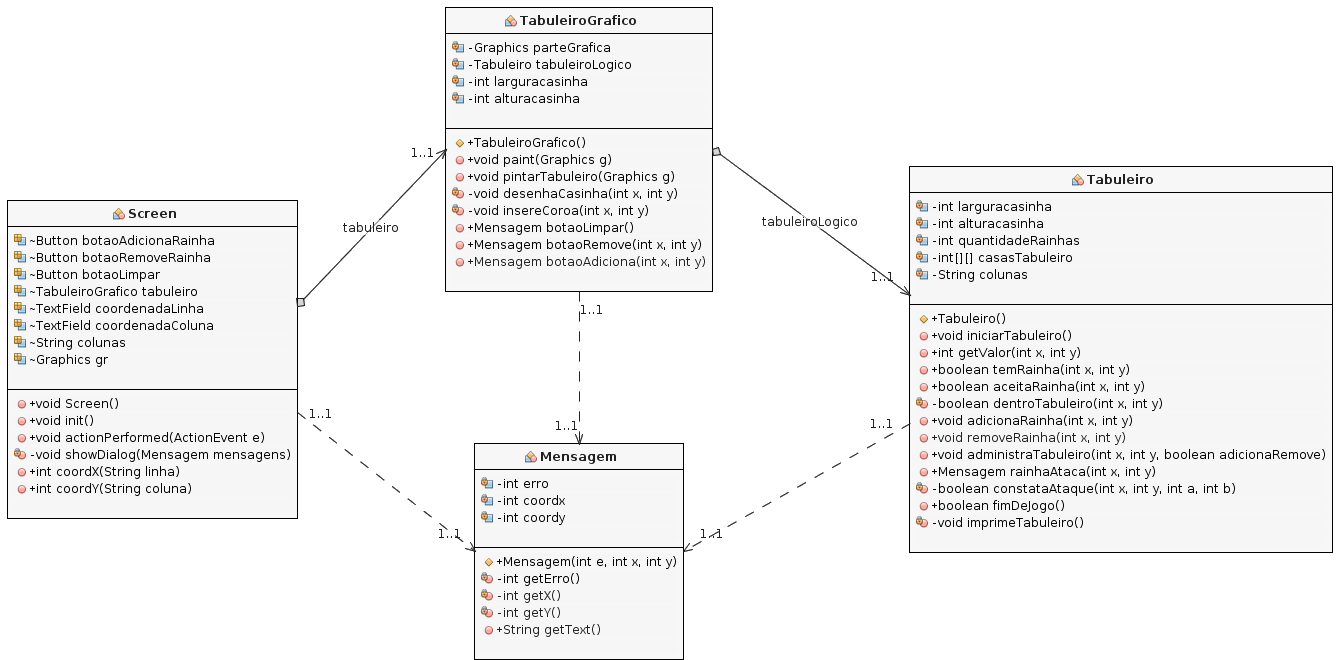
\includegraphics[width=1.0\textwidth]{./figures/diagrama-classe.png} % <- formatos PNG, JPG e PDF
	\caption{Diagrama de classes}
\end{figure}

\section{Utilizando BlueJ}

\begin{figure}[!htb]
	\centering
	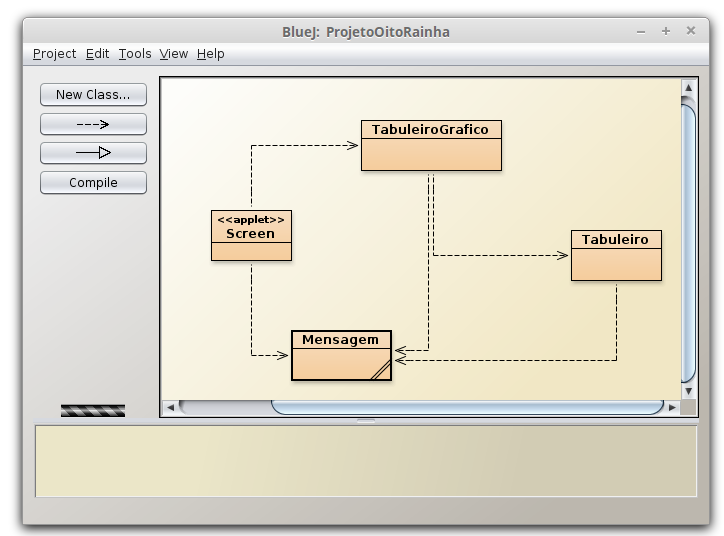
\includegraphics[width=0.4\textwidth]{./figures/diagrama-classe-bluej.png} % <- formatos PNG, JPG e PDF
	\caption{BlueJ tela}
\end{figure}


%\chapter{CONFIGURAÇÕES}
\section{Classe Screen}

\begin{lstlisting}
import java.applet.Applet;
import java.awt.*;
import java.awt.event.*;
import javax.swing.JOptionPane;
public class Screen extends Applet implements ActionListener {
    private Button botaoAdicionaRainha;
    private Button botaoRemoveRainha;
    private Button botaoLimpar;
	private TabuleiroGrafico tabuleiro;    
    private TextField coordenadaLinha;
    private TextField coordenadaColuna;
    private String colunas[] = {"-", "a","b","c","d","e","f","g","h"};
    private Graphics gr;
    public void Screen() {
        init();
    }
    @Override 
    public void init() {
        gr = this.getGraphics();
        botaoAdicionaRainha = new Button("adiciona");
        botaoRemoveRainha = new Button("remove");
        botaoLimpar = new Button("Limpar");
        tabuleiro = new TabuleiroGrafico();
        coordenadaLinha = new TextField(5);
        coordenadaColuna = new TextField(5);  
        setLayout(new BorderLayout());
        setSize(800, 600);
        setBackground(Color.white);
        add("Center", tabuleiro);   
        Panel bPanel = new Panel();
        add("South", bPanel);  
        bPanel.setLayout(new GridLayout(1,6));
        bPanel.add(new Label(" Coluna de a - h"));
        bPanel.add(coordenadaLinha);    
        bPanel.add(new Label(" Linha de 1-8"));
        bPanel.add(coordenadaColuna);   
        bPanel.add(botaoAdicionaRainha);
        bPanel.add(botaoRemoveRainha);
        bPanel.add(new Label(" "));
        bPanel.add(botaoLimpar);
        bPanel.setBackground(Color.BLACK);
        bPanel.setForeground(Color.YELLOW);
        botaoRemoveRainha.addActionListener(this);
        botaoAdicionaRainha.addActionListener(this);
        botaoLimpar.addActionListener(this);
        JOptionPane.showMessageDialog(null, "Oito  Rainhas desafio logico de dispor oito peças em um tabuleiro de forma que nenhuma seja atacada por outra. \n + Assim, faz-se necessário que duas rainhas quaisquer não estejam numa mesma linha, coluna ou diagonal.\n");        
    }
    @Override
    public void actionPerformed(ActionEvent e) { 
        String linha = coordenadaLinha.getText();
        String coluna = coordenadaColuna.getText();
        coordenadaLinha.setText("");
        coordenadaColuna.setText(""); 
        int x = coordX(linha);
        int y = coordY(coluna);
        if (e.getSource() == botaoLimpar) { 
            showDialog(tabuleiro.botaoLimpar());
            
        } else if (e.getSource() == botaoAdicionaRainha) {             
            showDialog(tabuleiro.botaoAdiciona(x, y));

        } else if (e.getSource() == botaoRemoveRainha) {                   
            showDialog(tabuleiro.botaoRemove(x, y));
        }
    }
    private void showDialog(Mensagem mensagens) {
        if (mensagens.getText().equals("ok"))
        {
            return;
        }
        JOptionPane.showMessageDialog(null, mensagens.getText());    
    }
    public int coordX(String linha){
        switch( linha )
        {
            case "a": return 0;
            case "b": return 1;
            case "c": return 2;
            case "d": return 3;
            case "e": return 4;
            case "f": return 5;
            case "g": return 6;
            case "h": return 7;
            default: return -1;
        }    

    }
      public int coordY(String coluna){
        switch( coluna )
        {
            case "8": return 0;
            case "7": return 1;
            case "6": return 2;
            case "5": return 3;
            case "4": return 4;
            case "3": return 5;
            case "2": return 6;
            case "1": return 7;
            default: return -1;
        } 
    }
}
\end{lstlisting}
\newpage
\section{Classe TabuleiroGrafico}

\begin{lstlisting}
import java.awt.*;
public class TabuleiroGrafico extends Canvas 
{
    private Graphics parteGrafica;
    private Tabuleiro tabuleiroLogico;
    private int larguracasinha;
    private int alturacasinha; 
    public TabuleiroGrafico()
    {
        this.tabuleiroLogico = new Tabuleiro();
        this.parteGrafica = this.getGraphics();
    }
    @Override
    public void paint(Graphics g) {
        pintarTabuleiro(g);
    }   
    public void pintarTabuleiro(Graphics g) {
        parteGrafica = g;
        larguracasinha = getBounds().width/10;
        alturacasinha = getBounds().height/10;
        String colunas[] = {"-", "a","b","c","d","e","f","g","h"};
        String linhas[] = {"-","8","7","6","5","4","3","2","1"};
        for (int i = 0; i < 8; i++) {
            for (int j = 0; j < 8; j++) {
                desenhaCasinha(i,j);
            }
        }
        parteGrafica.setColor(Color.black);
        int deslocar = alturacasinha/4;
        for (int i = 1; i < 9; i++) { 
            parteGrafica.drawString(colunas[i], i*larguracasinha + larguracasinha/2, alturacasinha/2 + deslocar);
            parteGrafica.drawString(colunas[i], i*larguracasinha + larguracasinha/2, alturacasinha/2  + alturacasinha * 9);
            parteGrafica.drawString(linhas[i], larguracasinha/2 + deslocar, i*alturacasinha + alturacasinha/2 );
            parteGrafica.drawString(linhas[i], larguracasinha/2 -deslocar*2 + larguracasinha * 9, i*alturacasinha + alturacasinha/2 );
        }
    }
    private void desenhaCasinha(int x, int y) {
        int coresAlternadas = 0;
        parteGrafica.setColor(Color.yellow);
        parteGrafica.drawRect((x+1)*larguracasinha, (y+1)*alturacasinha, larguracasinha, alturacasinha); //(y+1) para transladar
        if ((x + y) % 2 == 0) {    
            coresAlternadas = 10;
        }     
        switch (tabuleiroLogico.getValor(x, y)) {
            case 0:
                parteGrafica.setColor(new Color(230+coresAlternadas, 230+coresAlternadas, 230+coresAlternadas)); 
                break;
            case 1:
                parteGrafica.setColor(new Color(230+coresAlternadas, 230+coresAlternadas, 230+coresAlternadas)); 
              //parteGrafica.setColor(new Color(160,110,110)); //se quiser ver as dicas
                break;
            case 2:
                parteGrafica.setColor(new Color(0,0,0));
                break;
        }
        parteGrafica.fillRect((x+1)*larguracasinha+1, (y+1)*alturacasinha+1, larguracasinha-1, alturacasinha-1);
        insereCoroa(x, y);
    }
    private void insereCoroa(int x, int y)
    {
        if (tabuleiroLogico.getValor(x, y) != 2) {
            return;
        }
        Dimension xy = getSize(); //Dimensoes padrão são 800 por 569 pra exibir coroa
        parteGrafica.setColor(Color.red);
        if (xy.width < 569 || xy.height < 569) {
            int coordx = (x+1)*larguracasinha + (larguracasinha-6)/2;
            int coordy = (y+1)*alturacasinha + (alturacasinha+6)/2;
            parteGrafica.drawString("W", coordx, coordy);                                            
            return;
        }
        int mediaa = (larguracasinha - 50)/2; 
        int mediab = (alturacasinha - 50)/2;
        int a = (x+1)*larguracasinha + mediaa;
        int b = (y+1)*alturacasinha + mediab;
        parteGrafica.drawLine(a+5, b+45, a+45, b+45);
        parteGrafica.drawLine(a+5, b+45, a+5, b+5);
        parteGrafica.drawLine(a+45, b+45, a+45, b+5);
        parteGrafica.drawLine(a+5, b+35, a+45, b+35);
        parteGrafica.drawLine(a+5, b+5, a+15, b+20);
        parteGrafica.drawLine(a+15, b+20, a+25, b+5);
        parteGrafica.drawLine(a+25, b+5, a+35, b+20);
        parteGrafica.drawLine(a+35, b+20, a+45, b+5);
        parteGrafica.drawOval(a+20, b+20, 10, 10);
    }
    public Mensagem botaoLimpar() { 
        parteGrafica = this.getGraphics();
        tabuleiroLogico.iniciarTabuleiro();
        pintarTabuleiro(parteGrafica);
        return new Mensagem(0,0,0); 
    }
    public Mensagem botaoRemove(int x, int y) {
        parteGrafica = this.getGraphics();
        if (x < 0 || y < 0) {
            return new Mensagem(99,0,0);  
        }
        if (tabuleiroLogico.temRainha(x, y)) {
            tabuleiroLogico.removeRainha(x, y);
            pintarTabuleiro(parteGrafica);
        } else {
            return new Mensagem(5,x,y);
        }            
        return new Mensagem(0,0,0);
    }
    public Mensagem botaoAdiciona(int x, int y) {
        parteGrafica = this.getGraphics();
        if (x < 0 || y < 0) {
            return new Mensagem(99,0,0); 
        }   
        if (tabuleiroLogico.aceitaRainha(x, y)){
            tabuleiroLogico.adicionaRainha(x, y);         
            pintarTabuleiro(parteGrafica);
            if ( tabuleiroLogico.fimDeJogo() ) {
                return new Mensagem(100,0,0);
            }
        } else {
           return tabuleiroLogico.rainhaAtaca(x,y);
        }
        return new Mensagem(0,0,0);
    }
}

\end{lstlisting}
\newpage
\section{Classe Tabuleiro}

\begin{lstlisting}
public class Tabuleiro {
    private int larguracasinha;
    private int alturacasinha;
    private int quantidadeRainhas = 0;
    private int[][] casasTabuleiro = new int[8][8];
    private String colunas[] = {"-", "a","b","c","d","e","f","g","h"};
    public Tabuleiro() {
        iniciarTabuleiro();   
        imprimeTabuleiro();
    }
    public void iniciarTabuleiro(){
        quantidadeRainhas = 0;
        for (int i = 0; i < 8; i++) {
            for (int j = 0; j < 8; j++) {
                casasTabuleiro[i][j] = 0;
            }
        }
    }
    public int getValor(int x, int y) {
        if (dentroTabuleiro(x,y)) {
            return casasTabuleiro[x][y];
        }
        return -1;
    }
    public boolean temRainha(int x, int y)
    {
        if (dentroTabuleiro(x,y) && casasTabuleiro[x][y] == 2)
        {
            return true;           
        }
        return false;
    }
    public boolean aceitaRainha(int x, int y)
    {
        if (dentroTabuleiro(x,y) && casasTabuleiro[x][y] == 0)
        {
           return true;
        }
       return false;
    }
    private boolean dentroTabuleiro(int x, int y) {
        return (x >= 0 && x < 8 && y >= 0 && y < 8);
    }
    public void adicionaRainha(int x, int y) {
        quantidadeRainhas++;
        casasTabuleiro[x][y] = 2;
        administraTabuleiro(x,y,true);     
        imprimeTabuleiro();
    }
    public void removeRainha(int x, int y) {
        casasTabuleiro[x][y] = 0;
        administraTabuleiro(x,y,false);
        quantidadeRainhas = 0; 
        for (int i = 0; i < 8; i++) {
            for (int j = 0; j < 8; j++) {
                if (casasTabuleiro[i][j] == 2) {
                    adicionaRainha(i,j);
                }
            }
        }
        imprimeTabuleiro();
    }
    public void administraTabuleiro(int x, int y, boolean adicionaRemove){
        int i, valor;
        if (adicionaRemove){
            valor = 1;
        } else {
            valor = 0;
        }
        for (i = 0; i < 8; i++) {
            if (i != y && casasTabuleiro[x][i] != 2) {
                casasTabuleiro[x][i] = valor;
            }
            if (i != x && casasTabuleiro[i][y] != 2) {    
            casasTabuleiro[i][y] = valor;
            }
        }
        for (i=1; dentroTabuleiro(x-i,y+i); i++) {
                casasTabuleiro[x-i][y+i] = valor;
        }
        for (i=1; dentroTabuleiro(x-i,y-i); i++) {
            casasTabuleiro[x-i][y-i] = valor;
        }
        for (i=1; dentroTabuleiro(x+i,y+i); i++) {
            casasTabuleiro[x+i][y+i] = valor;
        }
        for (i=1; dentroTabuleiro(x+i,y-i); i++) {
            casasTabuleiro[x+i][y-i] = valor;
        }
    }
    public Mensagem rainhaAtaca(int x, int y){
        int limitesupi = x;
        int limitesupj = y;
        int i = x; 
        int j = y; 
        if (dentroTabuleiro(x,y) && casasTabuleiro[x][y] == 2)
        {
            return new Mensagem(1, x, y);
        }
        for (int d = 1; d < 8; d++) {
            i--;
            j--;
            limitesupi++;
            limitesupj++;
            for (int z = i; z <= limitesupi; z++) {
                for (int w = j; w <= limitesupj; w++) {
                    if (dentroTabuleiro(z,w) && casasTabuleiro[z][w] == 2 && constataAtaque(x,y,z,w)){
                        return new Mensagem(2, z, w);
                    }
                }
            }
        }
        return new Mensagem(2, x, y);
    }
    private boolean constataAtaque(int x, int y, int a, int b)
    { 
      if (x == a || y == b )  {
          return true;
      }
      if ((x-a) == (y - b)){ 
          return true;
      }
      if ((-1)*(x-a) == (y -b)){ 
          return true; 
      }
      return false;
    }
    public boolean fimDeJogo(){
        return quantidadeRainhas == 8;
    }
    private void imprimeTabuleiro()
    {
        //System.out.println("Agora estamos com " + quantidadeRainhas + " rainha(s) no tabuleiro");
        for (int i = 0; i < 8; i++) {
            for (int j = 0; j < 8; j++) {
                //System.out.print(casasTabuleiro[i][j] + " ");
            }
            System.out.println(" ");
        }
    }   
}

\end{lstlisting}
\newpage
\section{Classe Mensagem}

\begin{lstlisting}
public class Mensagem {
    private final int erro;
    private final int coordx;
    private final int coordy;   
    public Mensagem(int e, int x, int y){
        this.coordx = x;
        this.coordy = y;
        this.erro = e;  
    }
    private int getErro(){
        return this.erro;
    }
    private int getX(){
        return this.coordx;
    }
    private int getY(){
        return this.coordy;
    }
    public String getText() {
        int e, x, y;
        e = getErro();
        x = getX();
        y = getY();
        String colunas[] = {"-", "a","b","c","d","e","f","g","h"};
        switch( e ) {
            case 0: 
              return "ok";
            case 1:
                return "Ja existe uma Rainha na coluna '" + colunas[x+1] + "' e na linha '" +  (8-y) +"'!";                  
            case 2:
                return "Existe conflito! Sofre ataque da Rainha da coluna '" + colunas[x+1] + "' e da linha '" +  (8-y) +"'";                  
            case 3: 
                return "Existe conflito na linha '" + colunas[x+1]  + "' e coluna '" + (8-y) + "' mas nao achamos com qual rainha ";                  
            case 5: 
                return "Nao existe rainha na coluna '" + colunas[x+1] + "' e linha '" + (8-y) + "'";                  
            case 99: 
                return "Valores invalidos para coluna ou linha!"; 
            case 100: 
               return "Parabens Voce conseguiu colocar as 8 rainhas!!"; 
            default:
               return "Valores invalidos!";
        }         
    }   
}
\end{lstlisting}

%--------------------------------------
%Elementos Pós-Textuais
%--------------------------------------

%Bibliografia, gerada automaticamente a partir do arquivo .bib em conjunto com as citações presentes no texto.
\clearpage
\addcontentsline{toc}{chapter}{Bibliography}
%\bibliographystyle{plainnat} 

\bibliographystyle{brazil}
\nocite{*}

\bibliography{bib/bibliografia}

%\chapter{Titulo do Anexo}

Isto \'e um exemplo de Anexo.



%Apendices. Use caso necessário. Todos capítulos após o comando \apendice serão tratados como Apêndices. 
%\apendice
%\chapter{Titulo do Ap\^endice}

Isto \'e um exemplo de Ap\^endice.


%\chapter{Titulo do Outro Ap\^endice}

Isto \'e um exemplo de Ap\^endice (b).



%Anexos. Use caso necessário. Todos capítulos após o comando \anexo serao tratados como Anexos. 
%\anexo
%\input{src/anexo_a}
%\chapter{Titulo do Outro Anexo}

Isto \'e um exemplo de Anexo (b).







\end{document}
